TOUT REPRENDRE : besoin aussi de voir que sol max ne peut etre un ncycle convexe non ngone




Cette section va établir le fait \ref{nece-cond} affirmant qu'un \ngone\ maximisant son aire à périmètre fixé doit être, a minima, un \ngone\ régulier.


\begin{tcolorbox}
	\itshape\small
	Les cas $n = 3$ et $n = 4$ étant résolus, voir les faits \ref{iso-tri} et \ref{quadri}, dans toutes les preuves de cette section, nous supposerons $n \geq 5 $.
\end{tcolorbox}


% ----------------------- %



%
%
%
%
%
%
%
%
%
%
%
%Précisons la nature des solutions optimales données par le fait \ref{at-least-one} ci-dessus.
%
%
%\begin{fact} \label{at-least-one-convex}
%    Soit $n \in \NN_{\geq3}$ un naturel fixé.
%    Parmi tous les \ngones\ convexes de longueur $\ell$ fixée, non nulle, il en existe au moins un d'aire maximale.
%\end{fact}
%
%
%\begin{proof}
%	XXXX
%	
%	donne l'existence, parmi tous les \ncycles\ convexes de longueur $\ell$, d'au moins un \ncycle\ $\setproba{M} = A_1 A_2 \cdots A_n$ d'aire algébrique maximale.
%	%
%	\begin{itemize}
%        \item $\sarea{\setproba{P}} \geq 0$ pour tout \ngone\ positif $\setproba{P}$ selon le fait \ref{sarea-ngone}, 
%        et de plus
%        $\area{\setproba{P}} = \abs{\sarea{\setproba{P}}}$ pour tout \ngone\ $\setproba{P}$ selon le fait \ref{sarea-ngone},
%        donc $\sarea{\setproba{M}}$ est supérieure, ou égale, à l'aire, géométrique, de tout \ngone\ convexe de longueur $\ell$.
%
%
%
%
%
%
%
%
%
%
%        \item Pour conclure, il suffit de démontrer que $\setproba{M}$ est un \ngone. Démontrons que le contraire est impossible.
%        %
%        \begin{enumerate}
%        	\item Supposons que trois sommets $A^{\,\prime}_i$, $A^{\,\prime}_{i+1}$ et $A^{\,\prime}_{i+2}$ soient alignés.
%			%
%			XXXX   DESSIN !
%			pas bon via triangle cassant la ligne des trois points
%			
%			
%        	\item Supposons l'existence de $(k, i) \in \ZintervalC{1}{n}^2$ où $k \neq i$ tel que $[A^{\,\prime}_i A^{\,\prime}_{i+1}]$ et $[A^{\,\prime}_k A^{\,\prime}_{k+1}]$ soient deux côtés non contigus sécants.
%			%
%			XXXX   DESSIN !
%			si se croise c'est cas plat mais rejeter avant
%
%
%        	\item Supposons l'existence de $(k, i) \in \ZintervalC{1}{n}^2$ où $k \neq i$ tel que $A^{\,\prime}_i = A^{\,\prime}_k$.
%			%
%			XXXX  Pb ici a priorir mais du coup on garde k gone au lieu de n gone, SI VRAI, on met en remarque que pas rave car on montrerea que n gone régulier meilleur que k gone régulier si n > k .
%        \end{enumerate}
%    \end{itemize}
%	
%	\null\vspace{-6ex}
%\end{proof}
%
%
%
%
%
%
%
%
%
%
%
%
%
%\begin{fact} \label{max-is-conv}
%    Si un \ncycle\ $\setproba{L}$ de longueur non nulle n'est pas un \ngone\ convexe, alors il existe un \ngone\ convexe $\setproba{P}$ tel que
%	$\cyclelen{\setproba{P}} = \cyclelen{\setproba{L}}$
%	et
%	$\geoarea{\setproba{P}} > \geoarea{\setproba{L}}$.
%\end{fact}
%
%
%\begin{proof}
%	Commençons par le cas \og hyper-dégénéré \fg: si tous les sommets de $\setproba{L}$ sont alignés, son aire géométrique est nulle. Le triangle équilatéral de côté $\frac13 \cyclelen{\setproba{L}}$ permet de conclure.
%	
%	Supposons maintenant que $\setproba{L}$ possède au moins trois sommets non alignés.
%	Notons $\setproba{C}$ l'enveloppe convexe de $\setproba{L}$ (nous savons donc que $\setproba{C}$ contient au moins un triangle).
%	
%	\begin{center}
%		\centering
%		\small\itshape
%		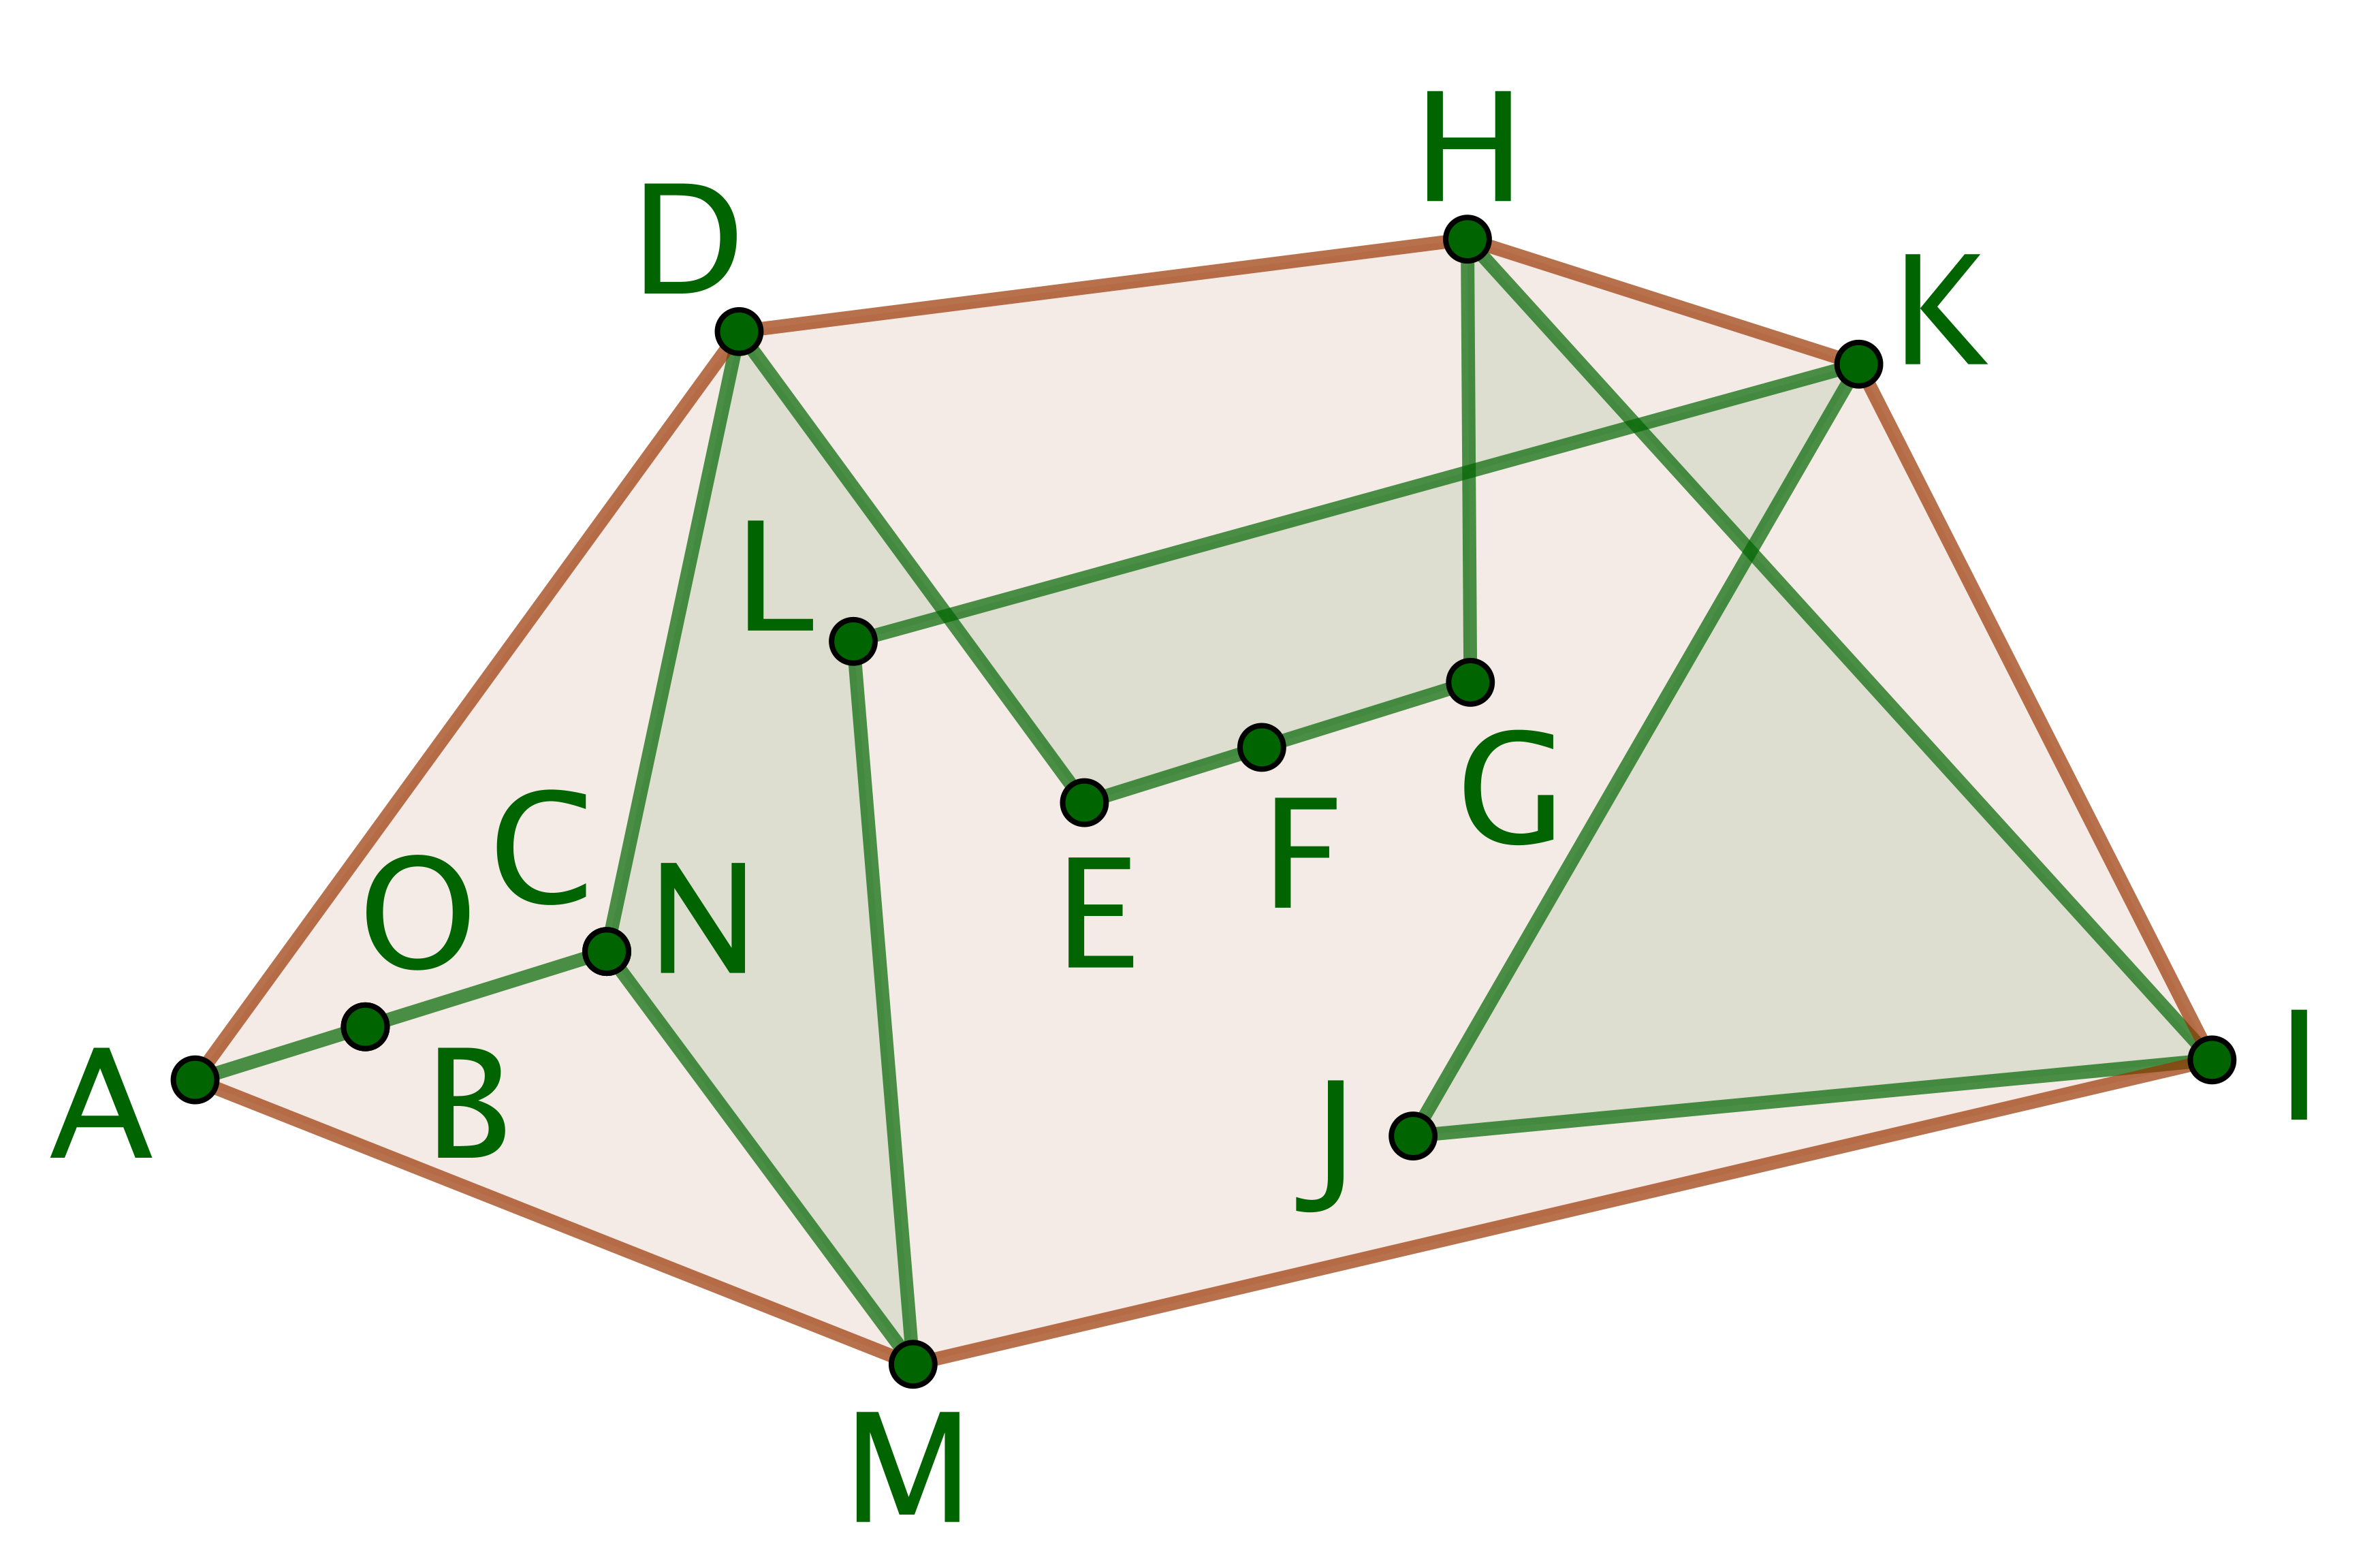
\includegraphics[scale=.45]{content/polygon/sol-is/convex-hull.png}
%		
%		\smallskip
%		Exemple où $N = C$ et $O = B$.
%	\end{center}
%	
%		
%	Clairement, $\cyclelen{\setproba{C}} < \cyclelen{\setproba{L}}$.
%	Quant à $\geoarea{\setproba{C}} > \geoarea{\setproba{L}}$, c'est une conséquence directe de la définition de l'aire géométrique combinée au fait que $\setproba{L}$ ne soit pas un \ngone\ convexe.
%	Il reste un problème à gérer: $\setproba{C}$ est un \xgone{s} avec $s \leq n$. 
%	%
%	Une idée simple, formalisée après, est d'ajouter des sommets assez prêts des côtés de $\setproba{C}$ pour garder la convexité, une longueur strictement inférieure à $\cyclelen{\setproba{L}}$, et une aire géométrique strictement plus grande que $\geoarea{\setproba{L}}$. Si c'est faisable, un agrandissement de rapport $r > 1$ donnera le \ngone\ $\setproba{P}$ cherché.
%	La figure suivante illustre cette idée.
%
%	\begin{center}
%		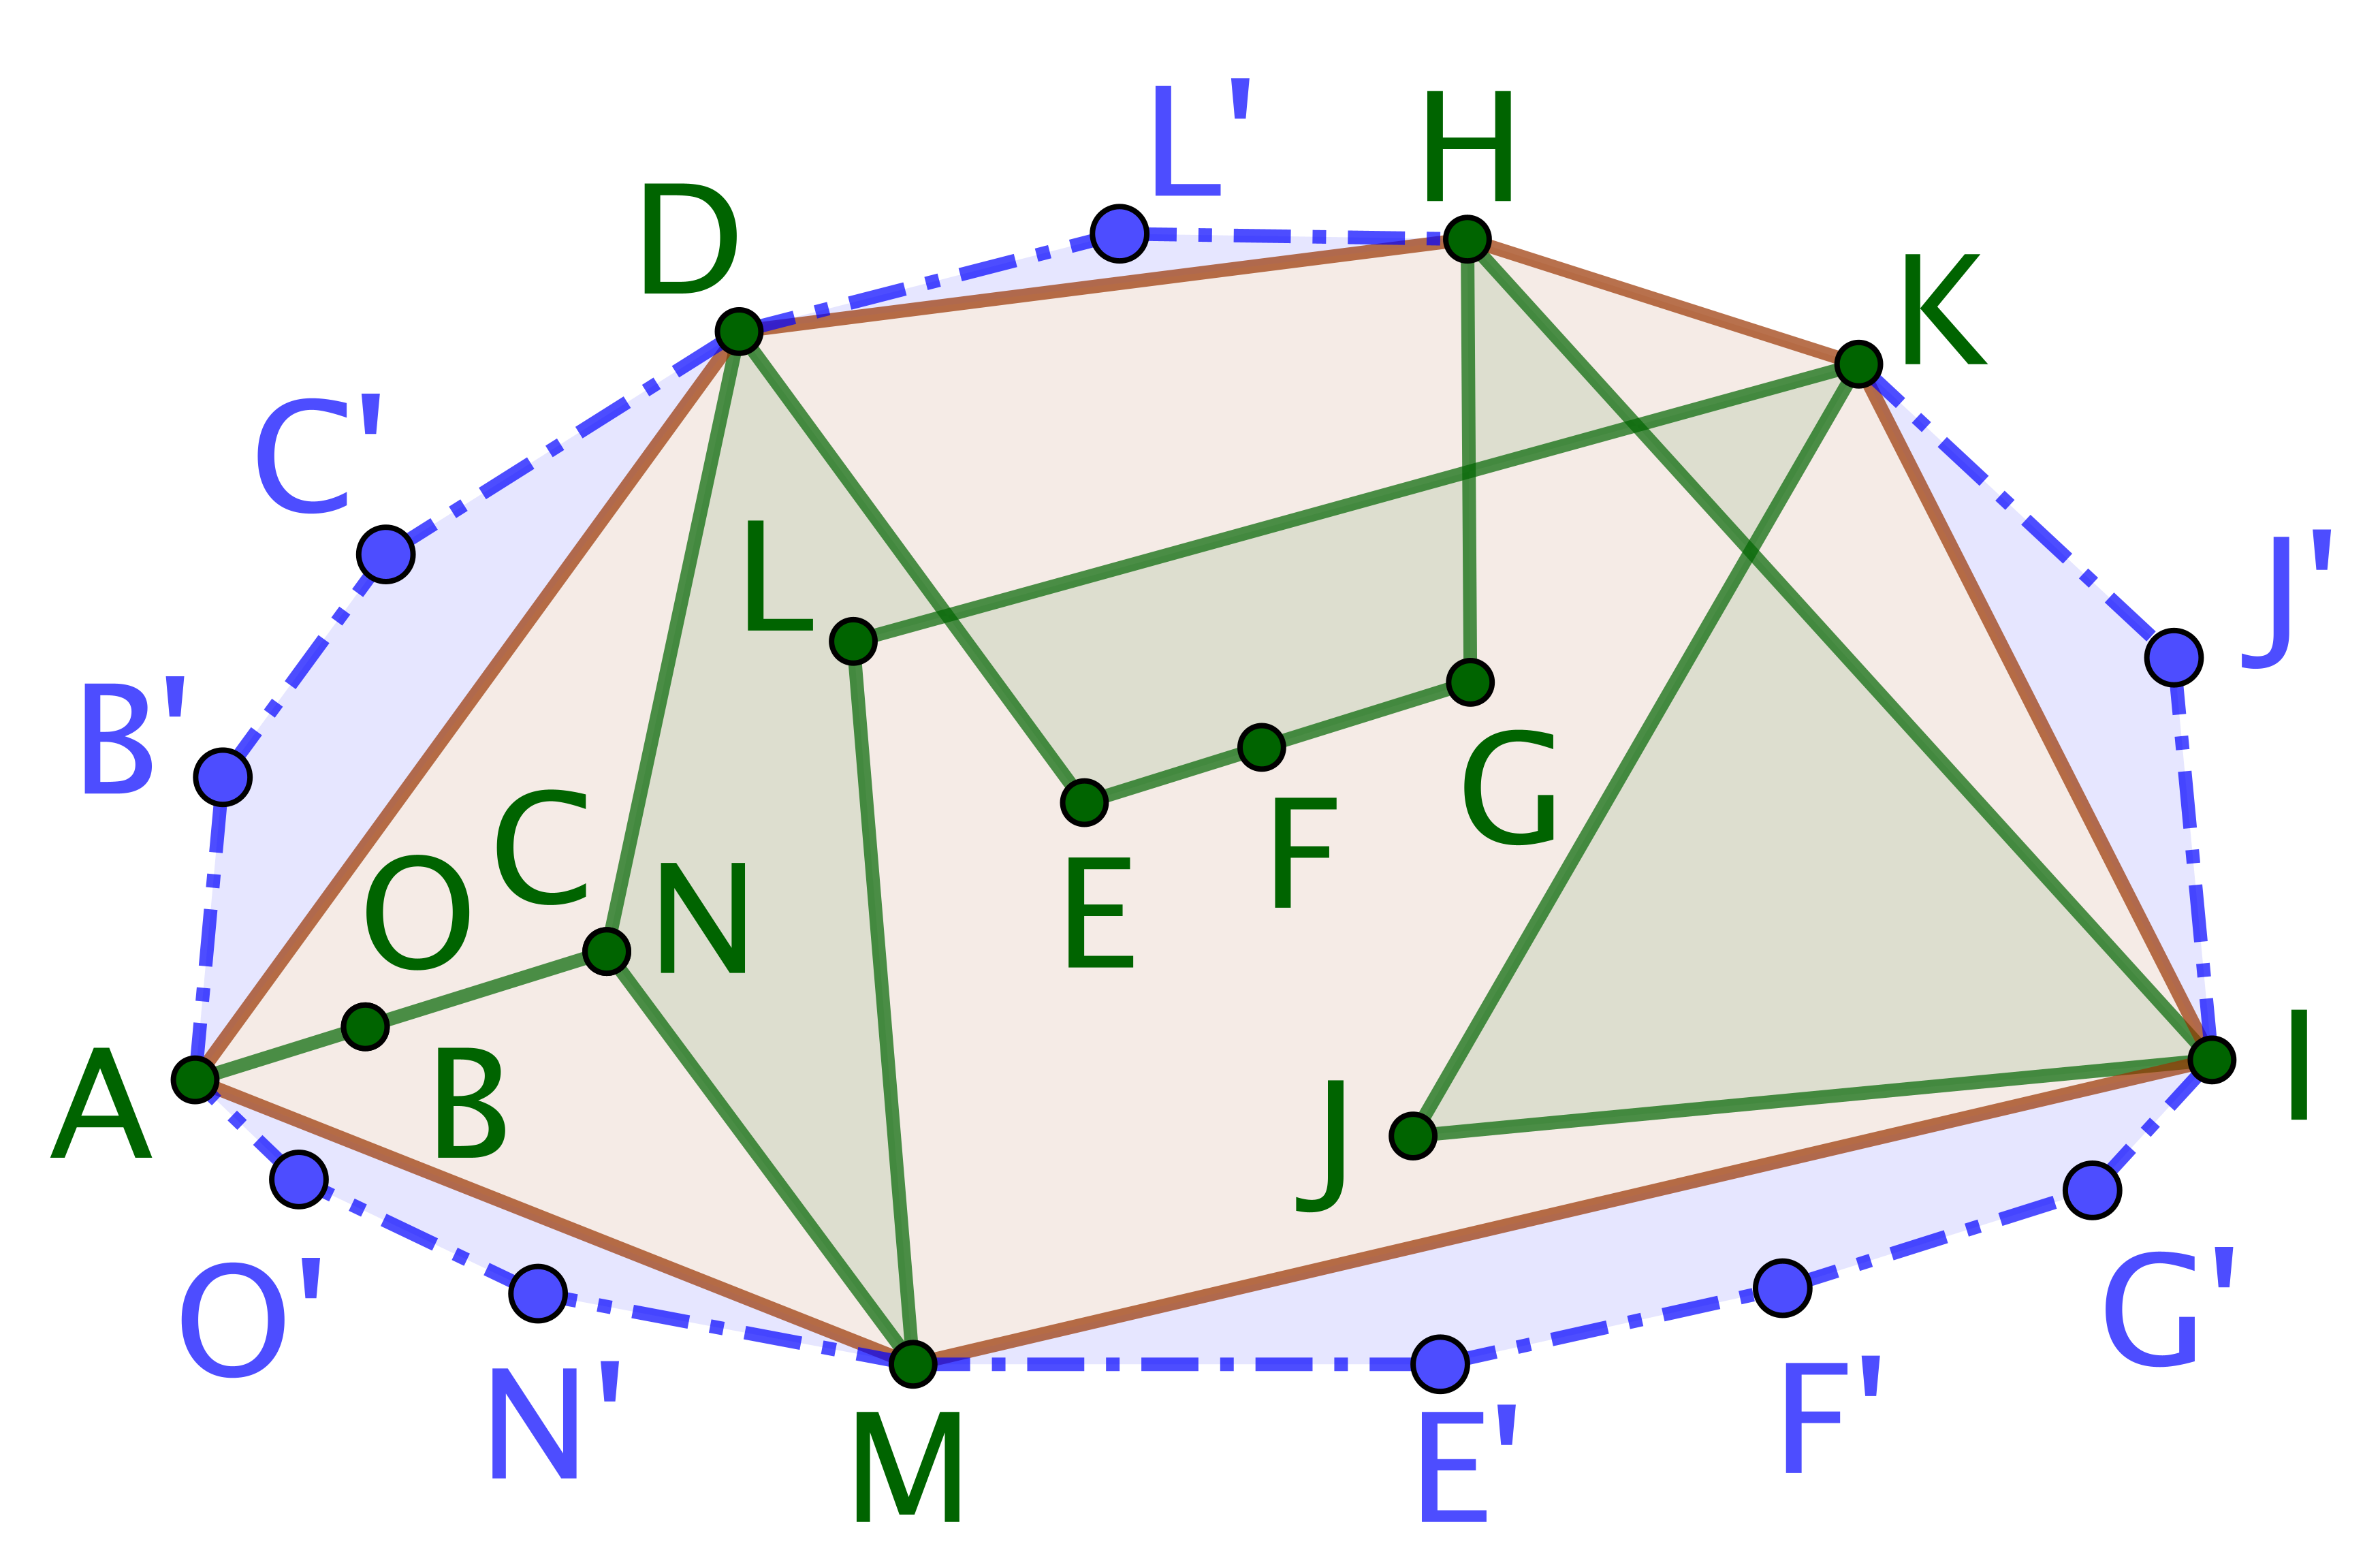
\includegraphics[scale=.45]{content/polygon/sol-is/convex-hull-distortion.png}
%	\end{center}
%
%
%	$m = n - s$ compte les sommets manquants.
%	Si $m = 0$, il n'y a rien à faire.
%	Sinon, posons $\delta = \frac{\cyclelen{\setproba{L}} - \cyclelen{\setproba{C}}}{m}$.
%	%
%	\begin{enumerate}
%		\item \label{add-vertex-start}
%		Considérons $[AB]$ un côté quelconque de $\setproba{C}$.
%		Les droites portées par les côtés \og \emph{autour} \fg\ de $[AB]$ \og \emph{dessinent} \fg\ une région contenant toujours un triangle $ABC$ dont l'intérieur est à l'extérieur
%		\footnote{
%			C'est ce que l'on appelle de la \og \emph{low poetry} \fg\,.
%		}
%		de $\setproba{C}$ comme dans les deux cas ci-dessous.
%	%
%		\begin{multicols}{2}
%			\centering
%
%			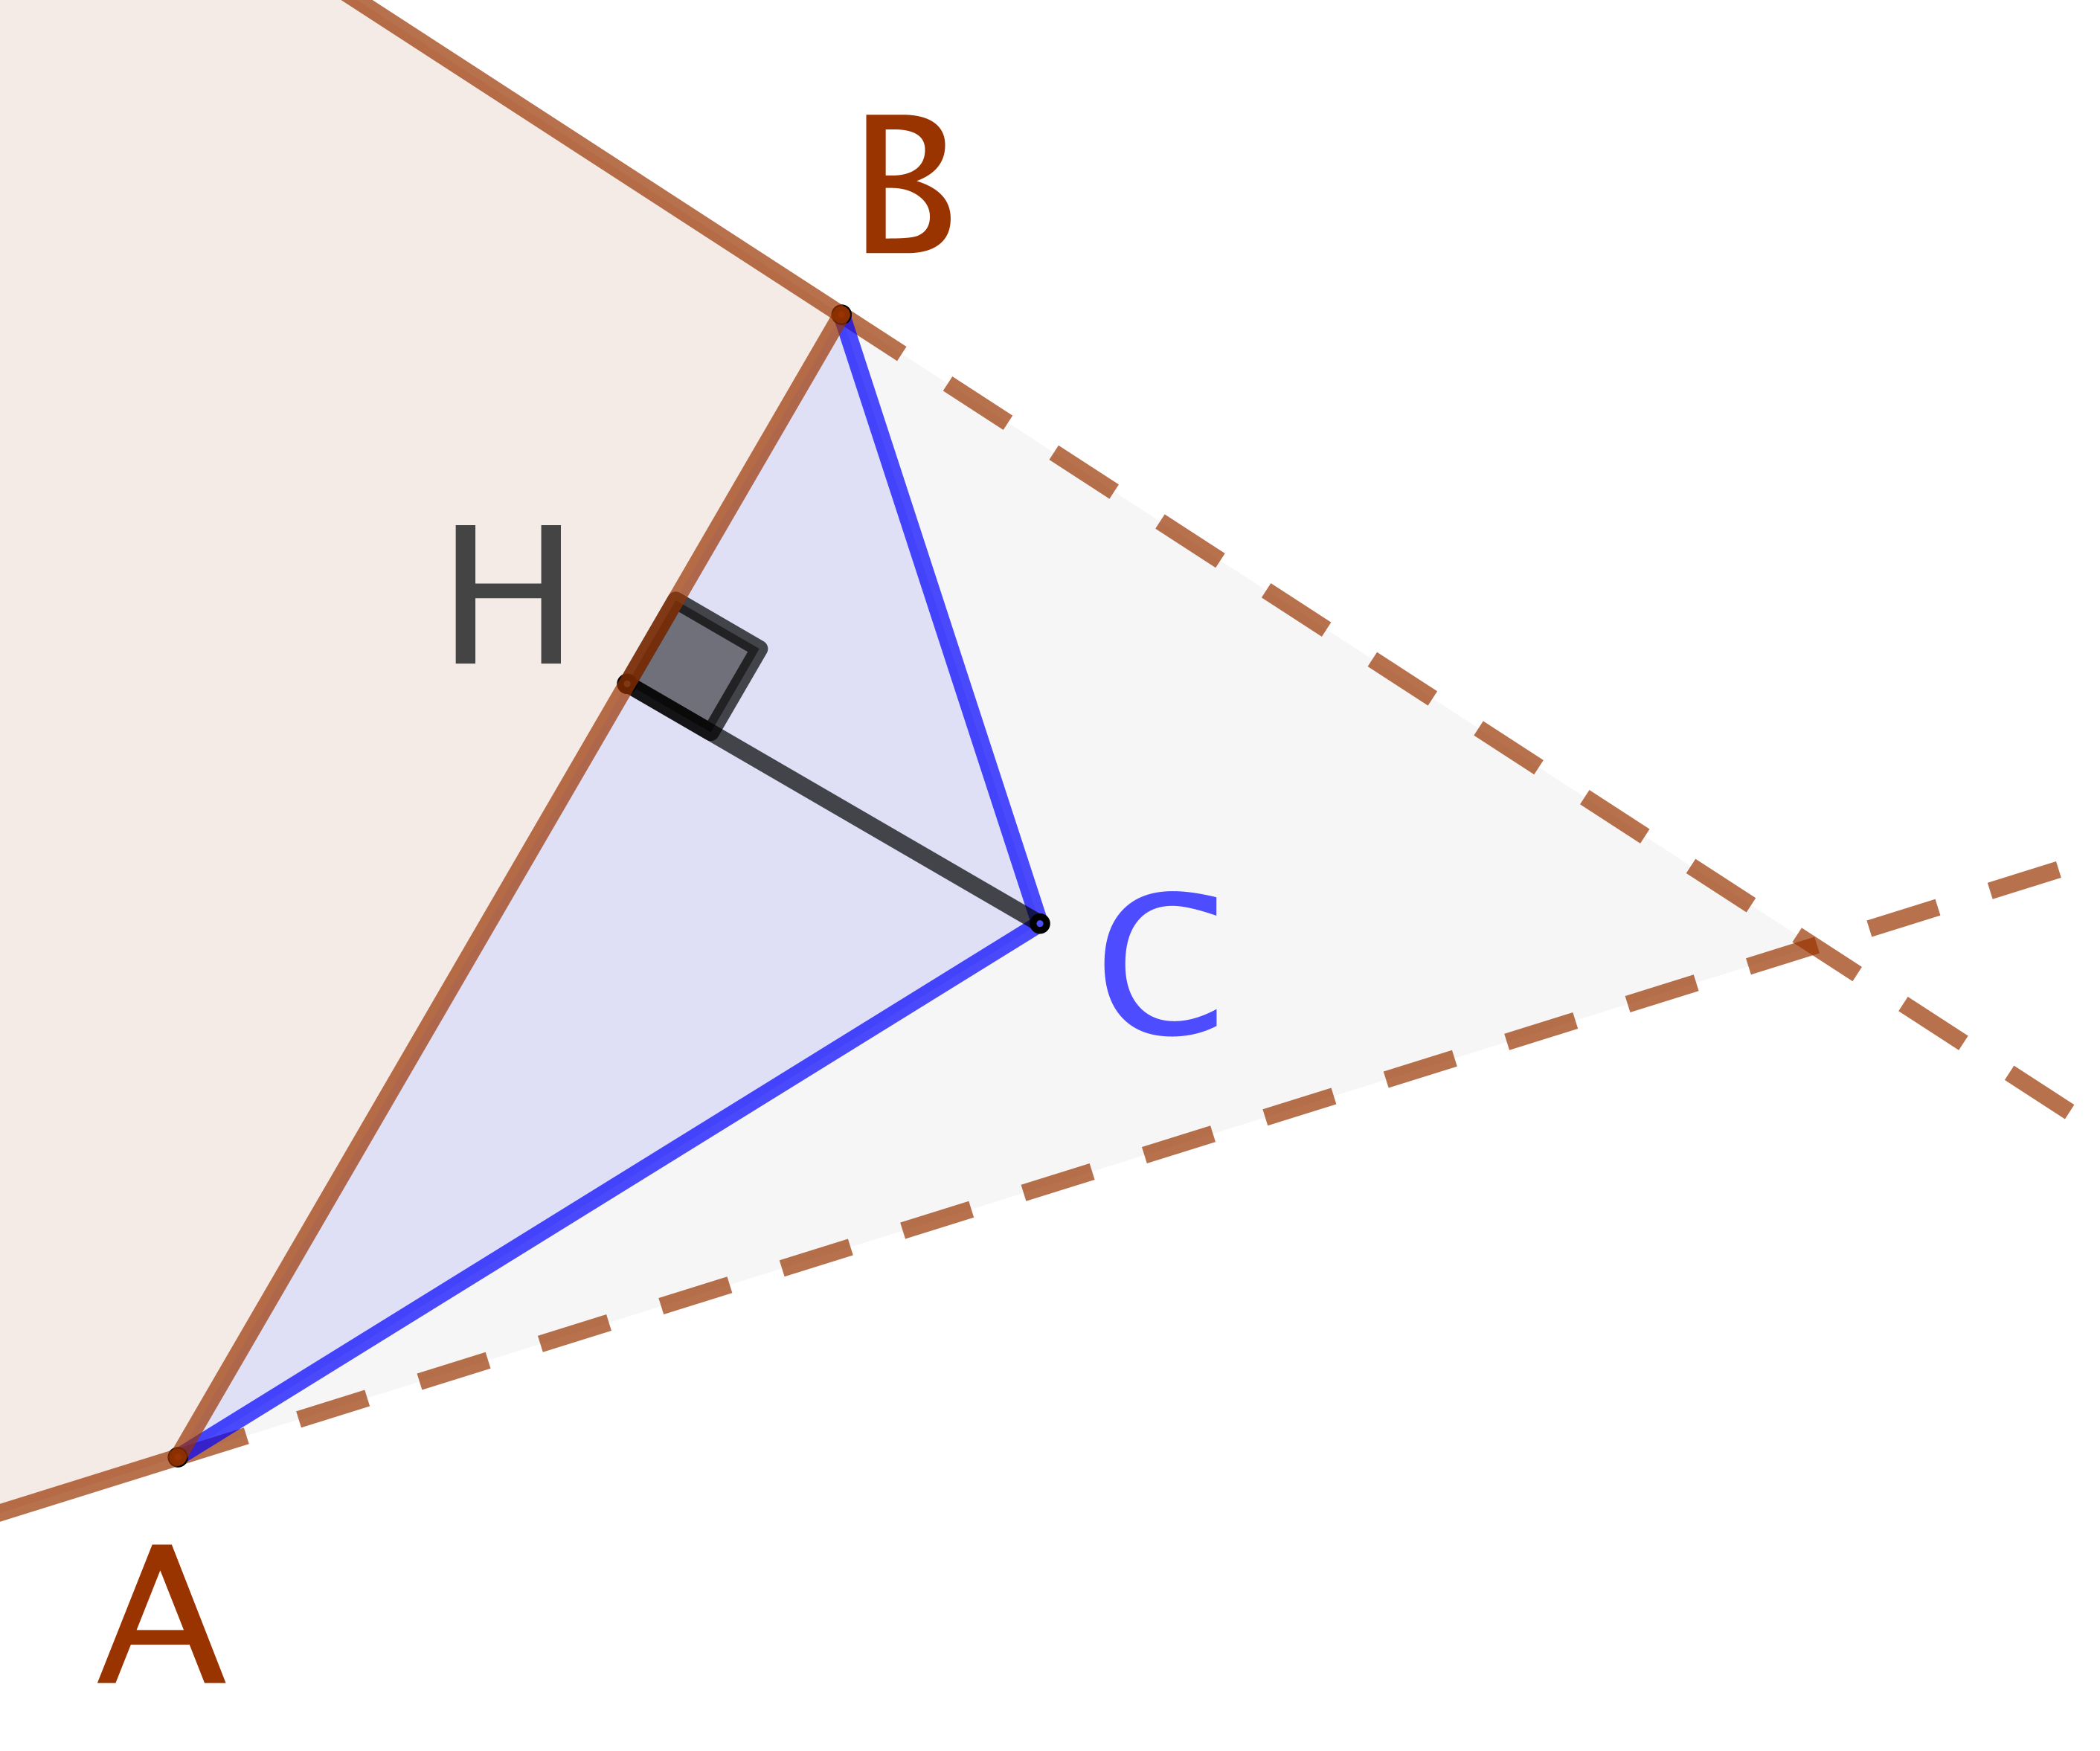
\includegraphics[scale=.35]{content/polygon/sol-is/add-vertex-1.png}
%
%			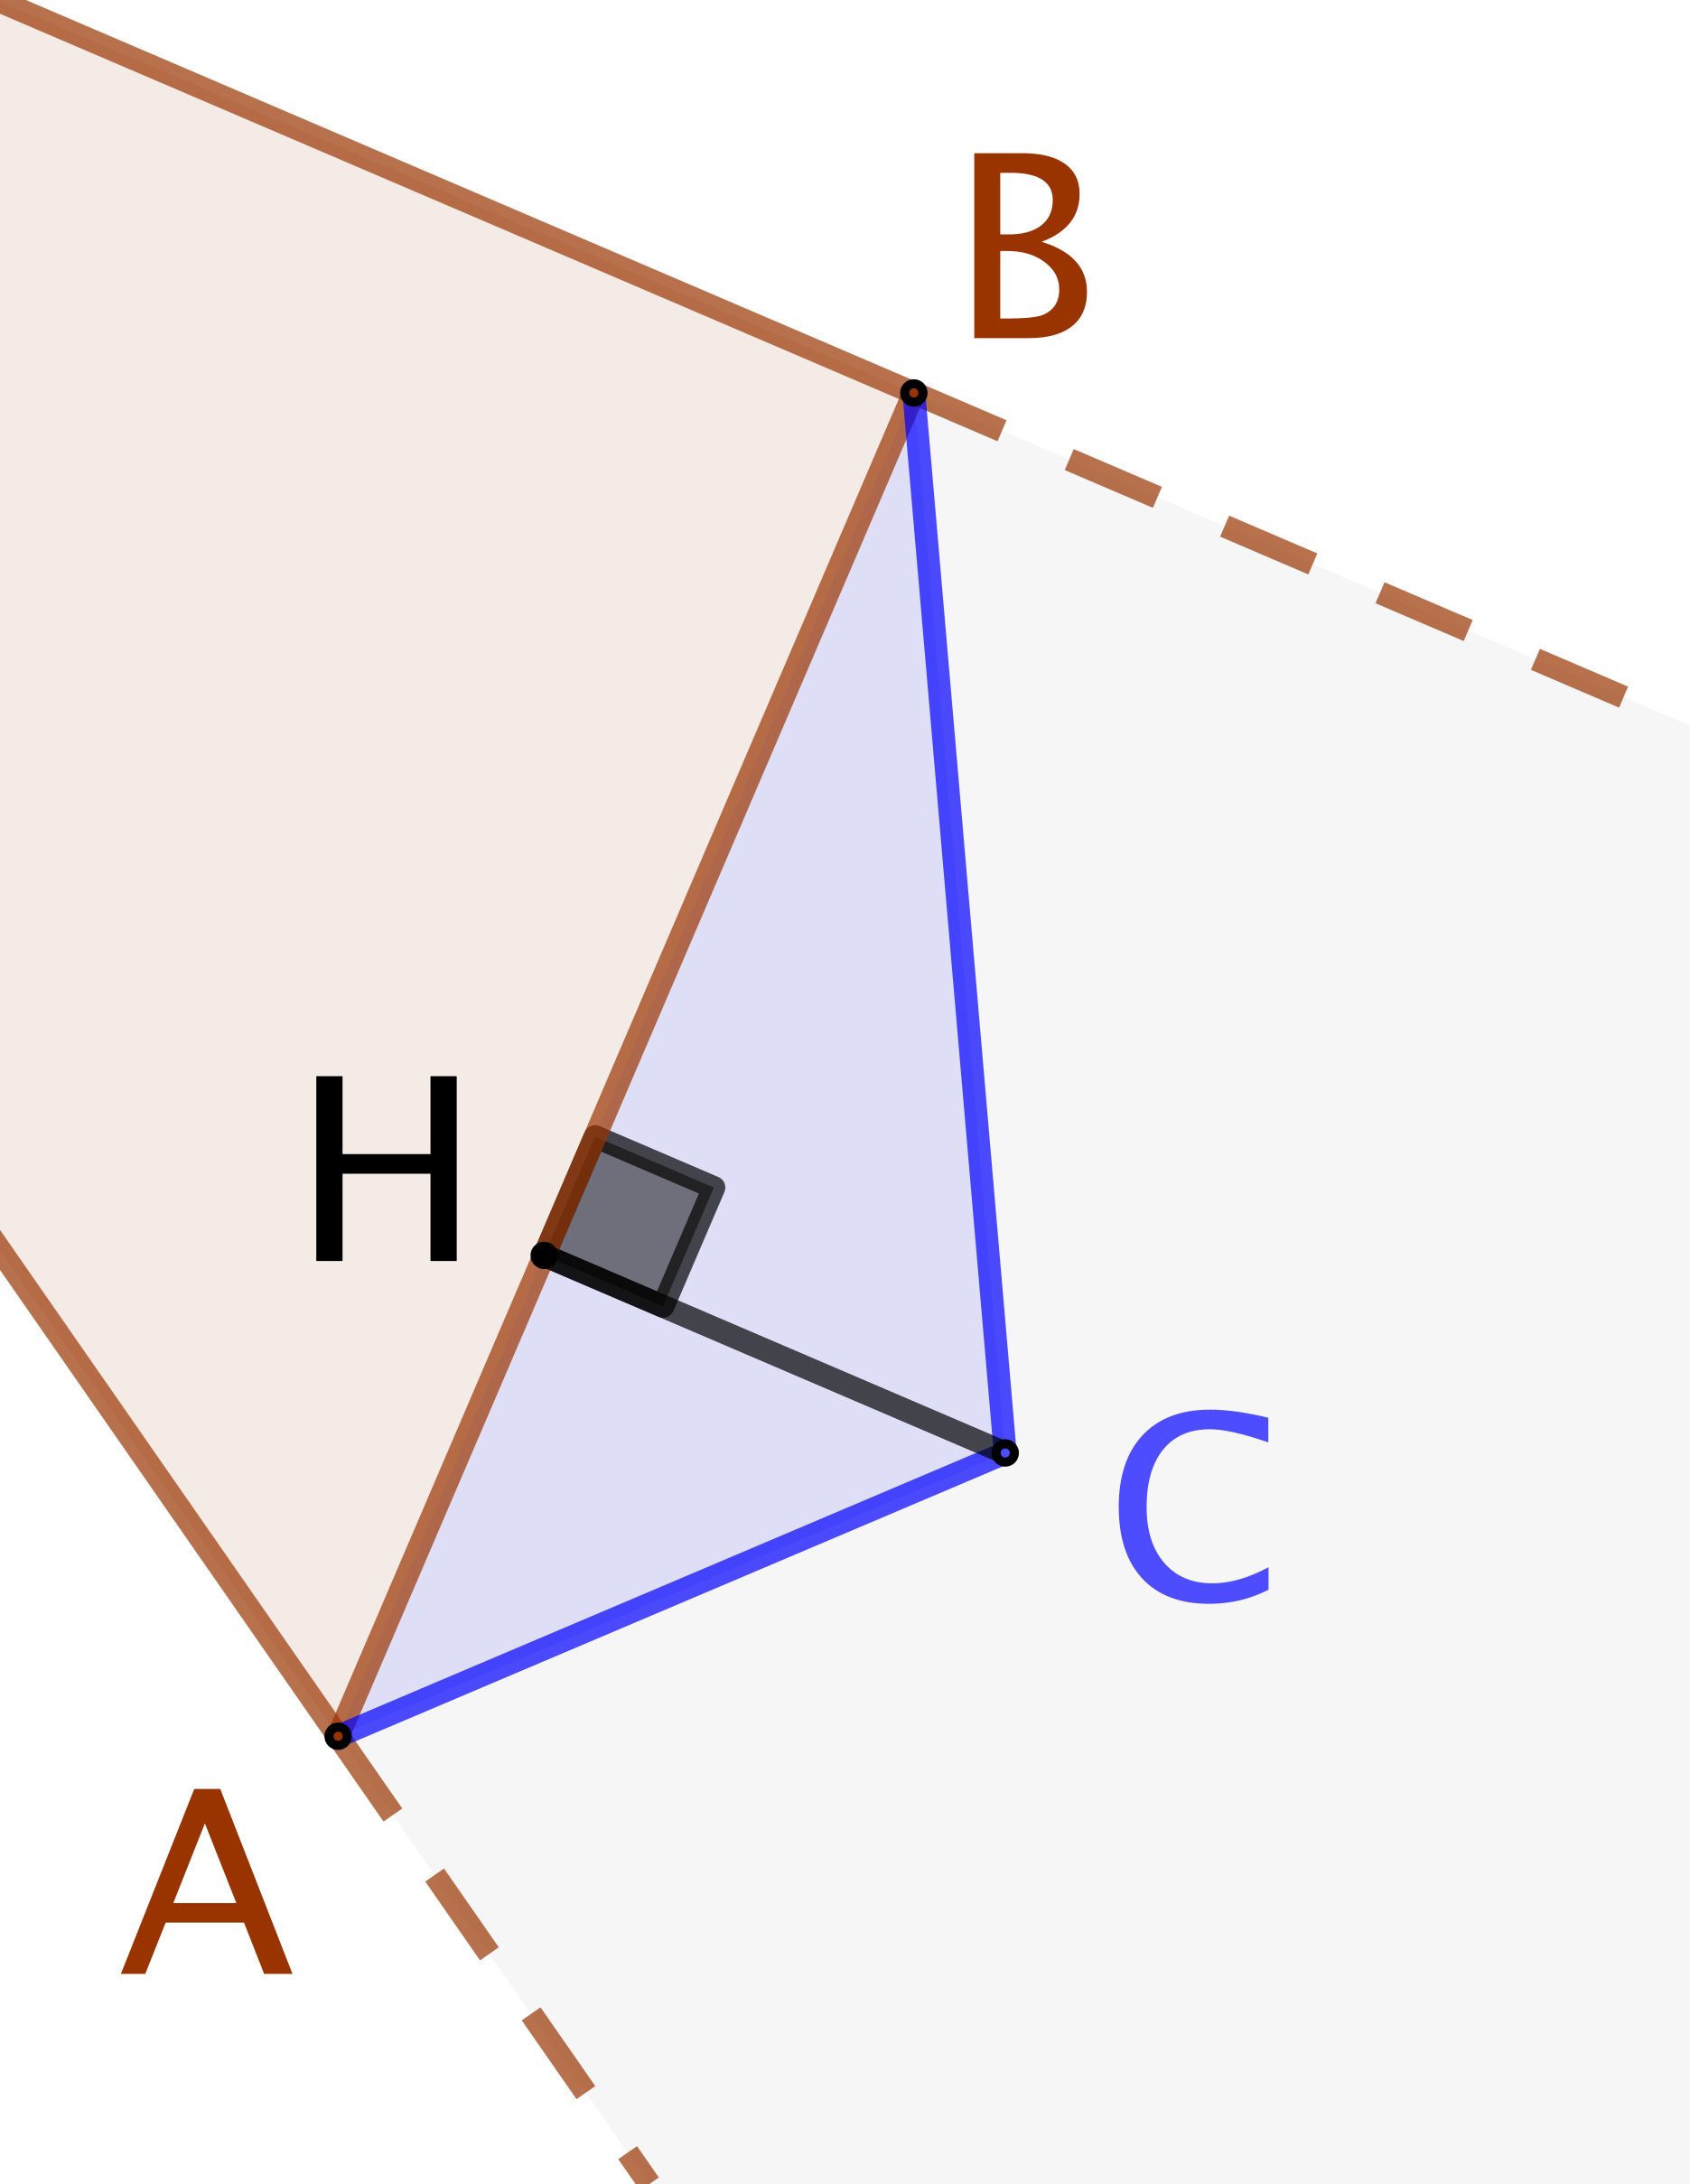
\includegraphics[scale=.35]{content/polygon/sol-is/add-vertex-2.png}
%		\end{multicols}
%
%		\item Clairement, le polygone $\setproba{C}_+$ obtenu à partir de $\setproba{C}$ en remplaçant le côté $[AB]$ par les côtés $[AC]$ et $[CB]$ est un convexe avec un sommet de plus que $\setproba{C}$.
%
%		\item \label{add-vertex-end}
%		Comme $HC$ peut être rendu aussi proche de $0$ que souhaité, il est aisé de voir que l'on peut choisir cette distance de sorte que $AC + BC < AB + \delta$.
%		Dès lors, le périmètre de $\setproba{C}_+$ augmente inférieurement strictement à $\delta$ relativement à $\setproba{C}$.
%
%		\item En répétant $(m-1)$ fois les étapes \ref{add-vertex-start} à \ref{add-vertex-end}, nous obtenons un \ngone\ convexe $\setproba{P}$ tel que
%		$\geoarea{\setproba{P}} > \geoarea{\setproba{L}}$
%		et
%		$\cyclelen{\setproba{P}} < \cyclelen{\setproba{C}} + m \delta = \cyclelen{\setproba{L}}$.
%	\end{enumerate}
%	
%	\null\vspace{-6ex}
%\end{proof}
%
%
%% ----------------------- %
%
%
%\begin{fact} \label{iso-poly}
%	Si un \ngone\ convexe $\setproba{P}$ n'est pas un \nequi, alors on peut construire un \ngone\ convexe $\setproba{P}^{\,\prime}$ tel que
%	$\cyclelen{\setproba{P}^{\,\prime}} = \cyclelen{\setproba{P}}$
%	et
%	$\area{\setproba{P}^{\,\prime}} > \area{\setproba{P}}$.
%\end{fact}
%
%
%\begin{proof}
%	Considérons un \ngone\ convexe $\setproba{P}$ qui ne soit pas un \nequi.
%	Dans ce cas, $\setproba{P}$ admet un triplet de sommets consécutifs $A$, $B$ et $C$ tels que $AB \neq BC$ (sinon, on obtiendrait de proche en proche un \nequi).
%	La construction vue dans la preuve du fait \ref{tri-one-side-fixed} nous donne la solution: voir les deux dessins ci-après dans lesquels $(AC) \parallel (BB^{\,\prime})$.
%	Pour le 2\ieme\ cas, il n'est pas possible d'utiliser le triangle $AB^{\,\prime}C$ isocèle en $B^{\,\prime}$ car $(B^{\,\prime}C)$ porte le côté de $\setproba{P}$ de sommet $C$ juste après $[BC]$, mais ce problème se contourne en considérant un point $B^{\,\prime\prime}$ du segment ouvert $]BB^{\,\prime}[$ (si besoin, se reporter au 2\ieme\ dessin de la preuve du fait \ref{tri-one-side-fixed}).
%	%
%	\begin{multicols}{2}
%		\centering
%
%		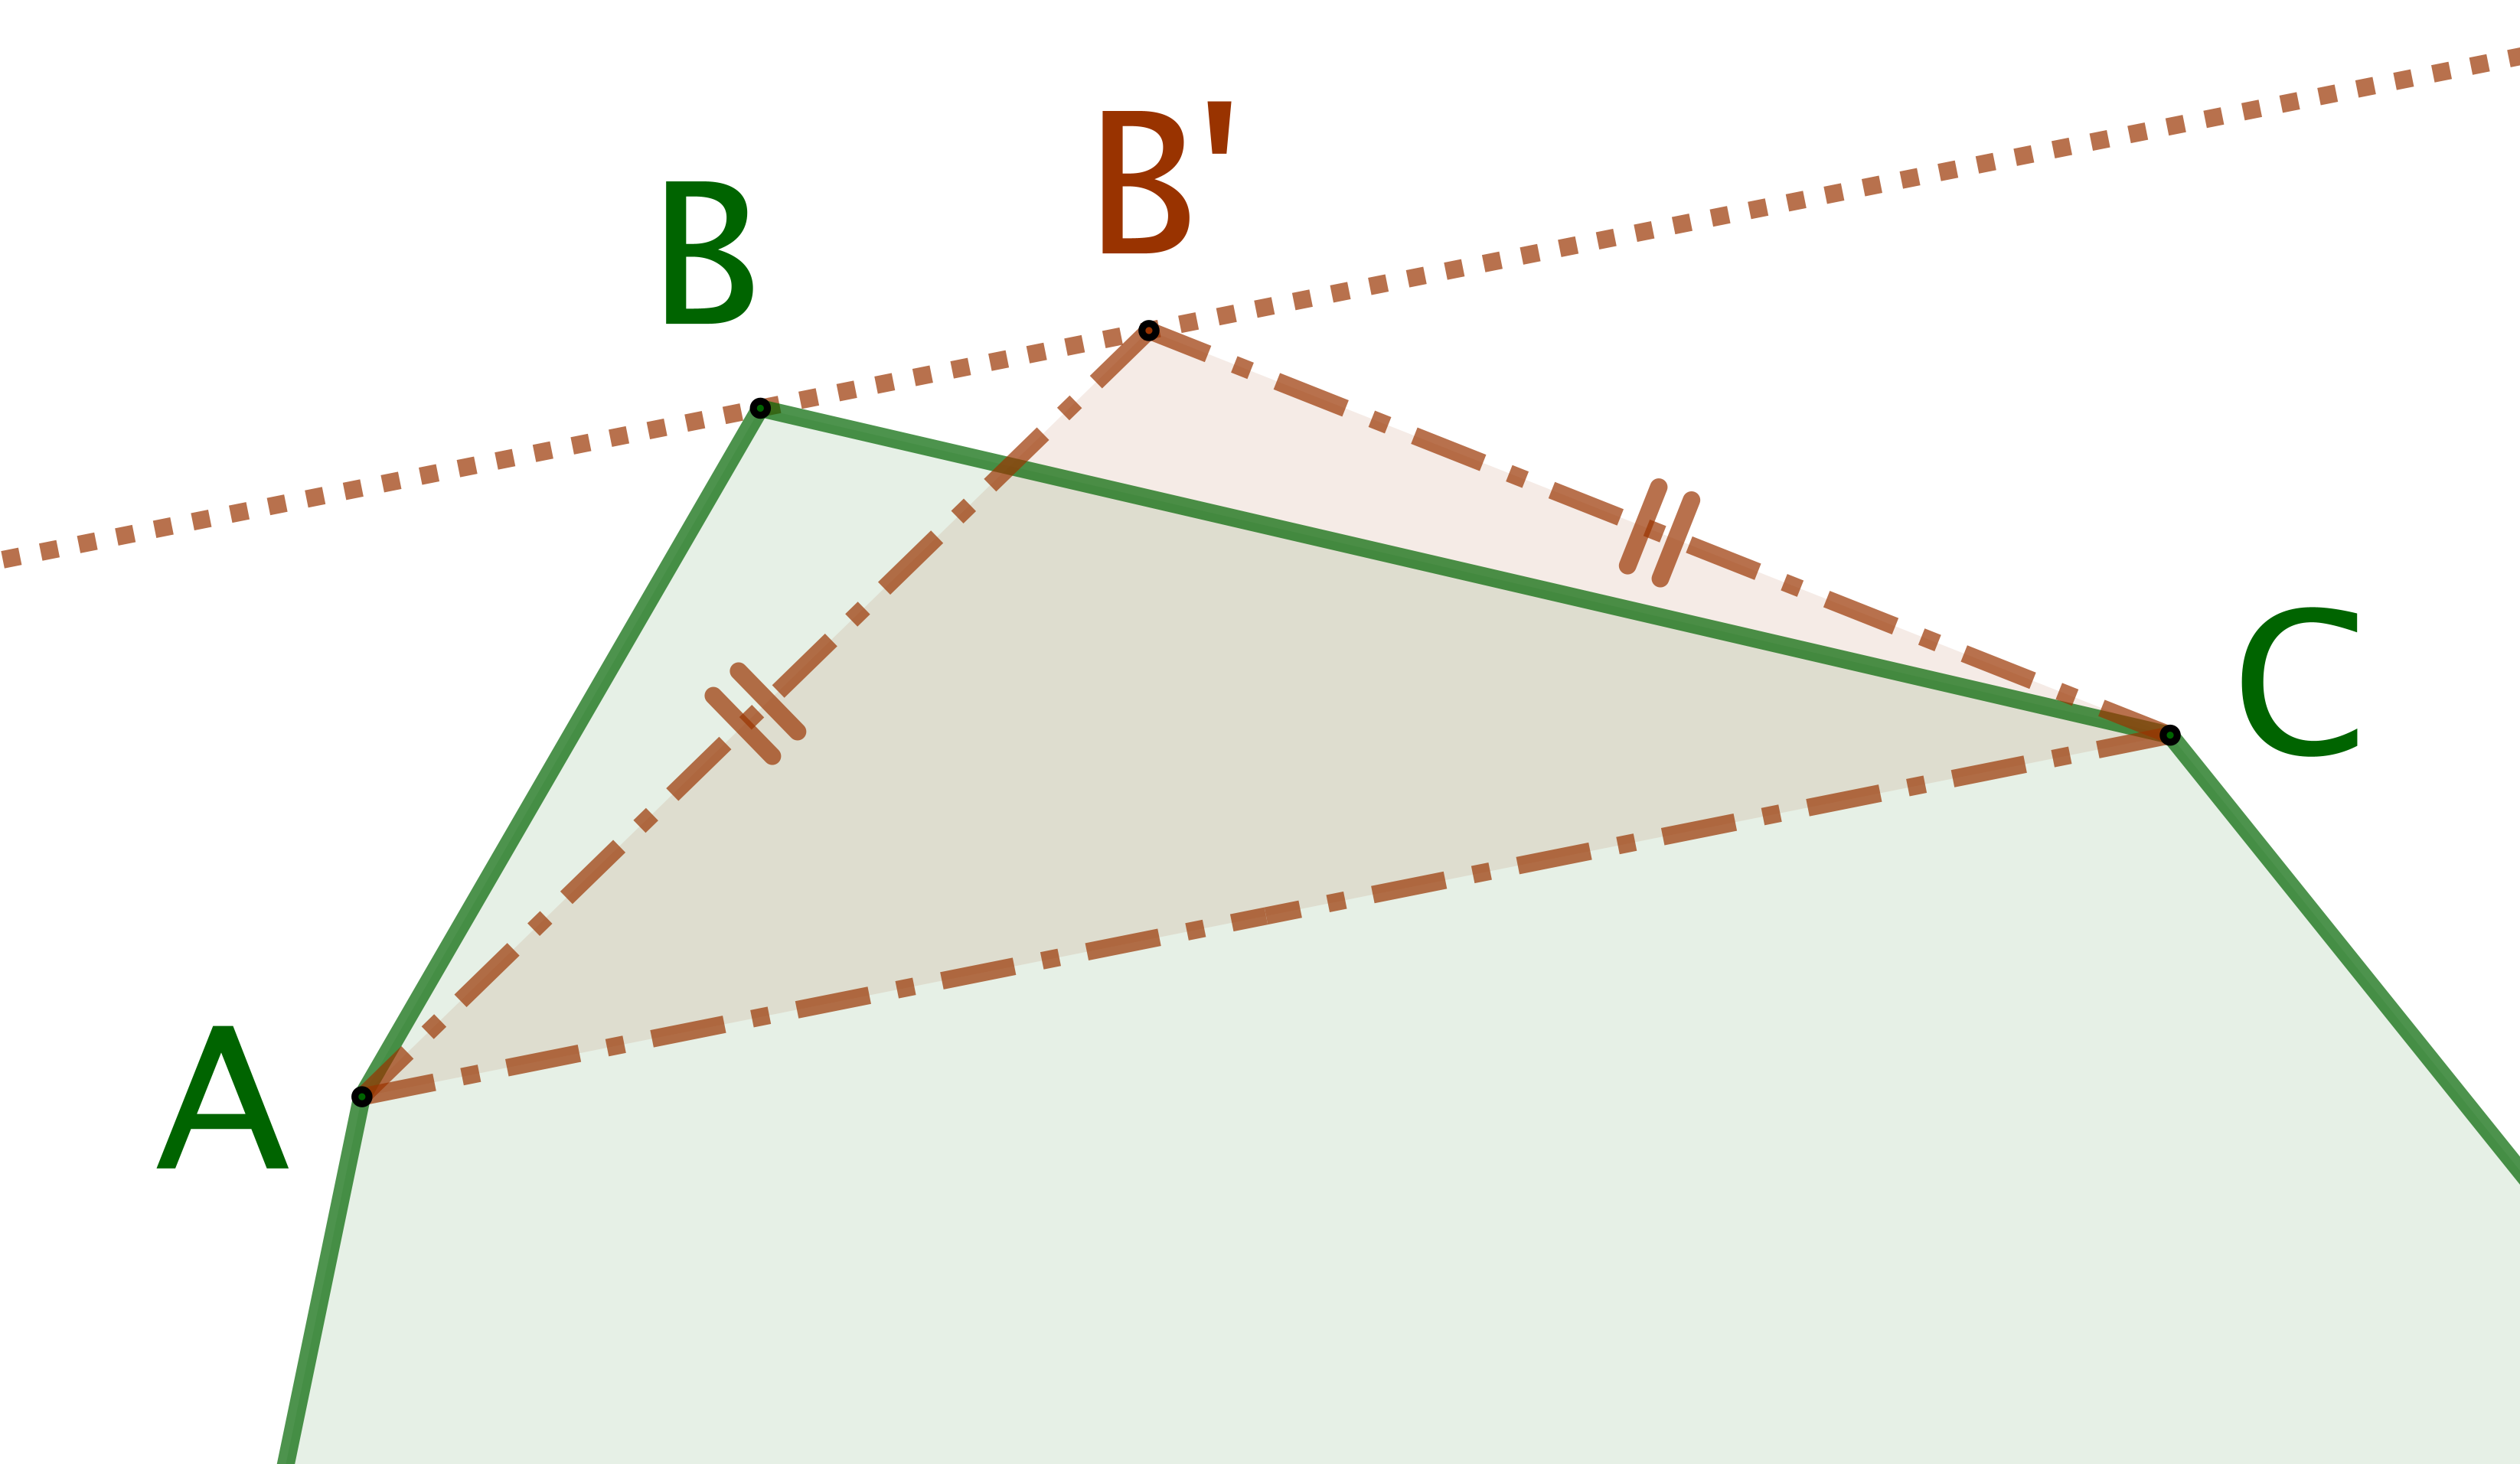
\includegraphics[scale=.4]{content/polygon/sol-is/not-iso-OK.png}
%
%		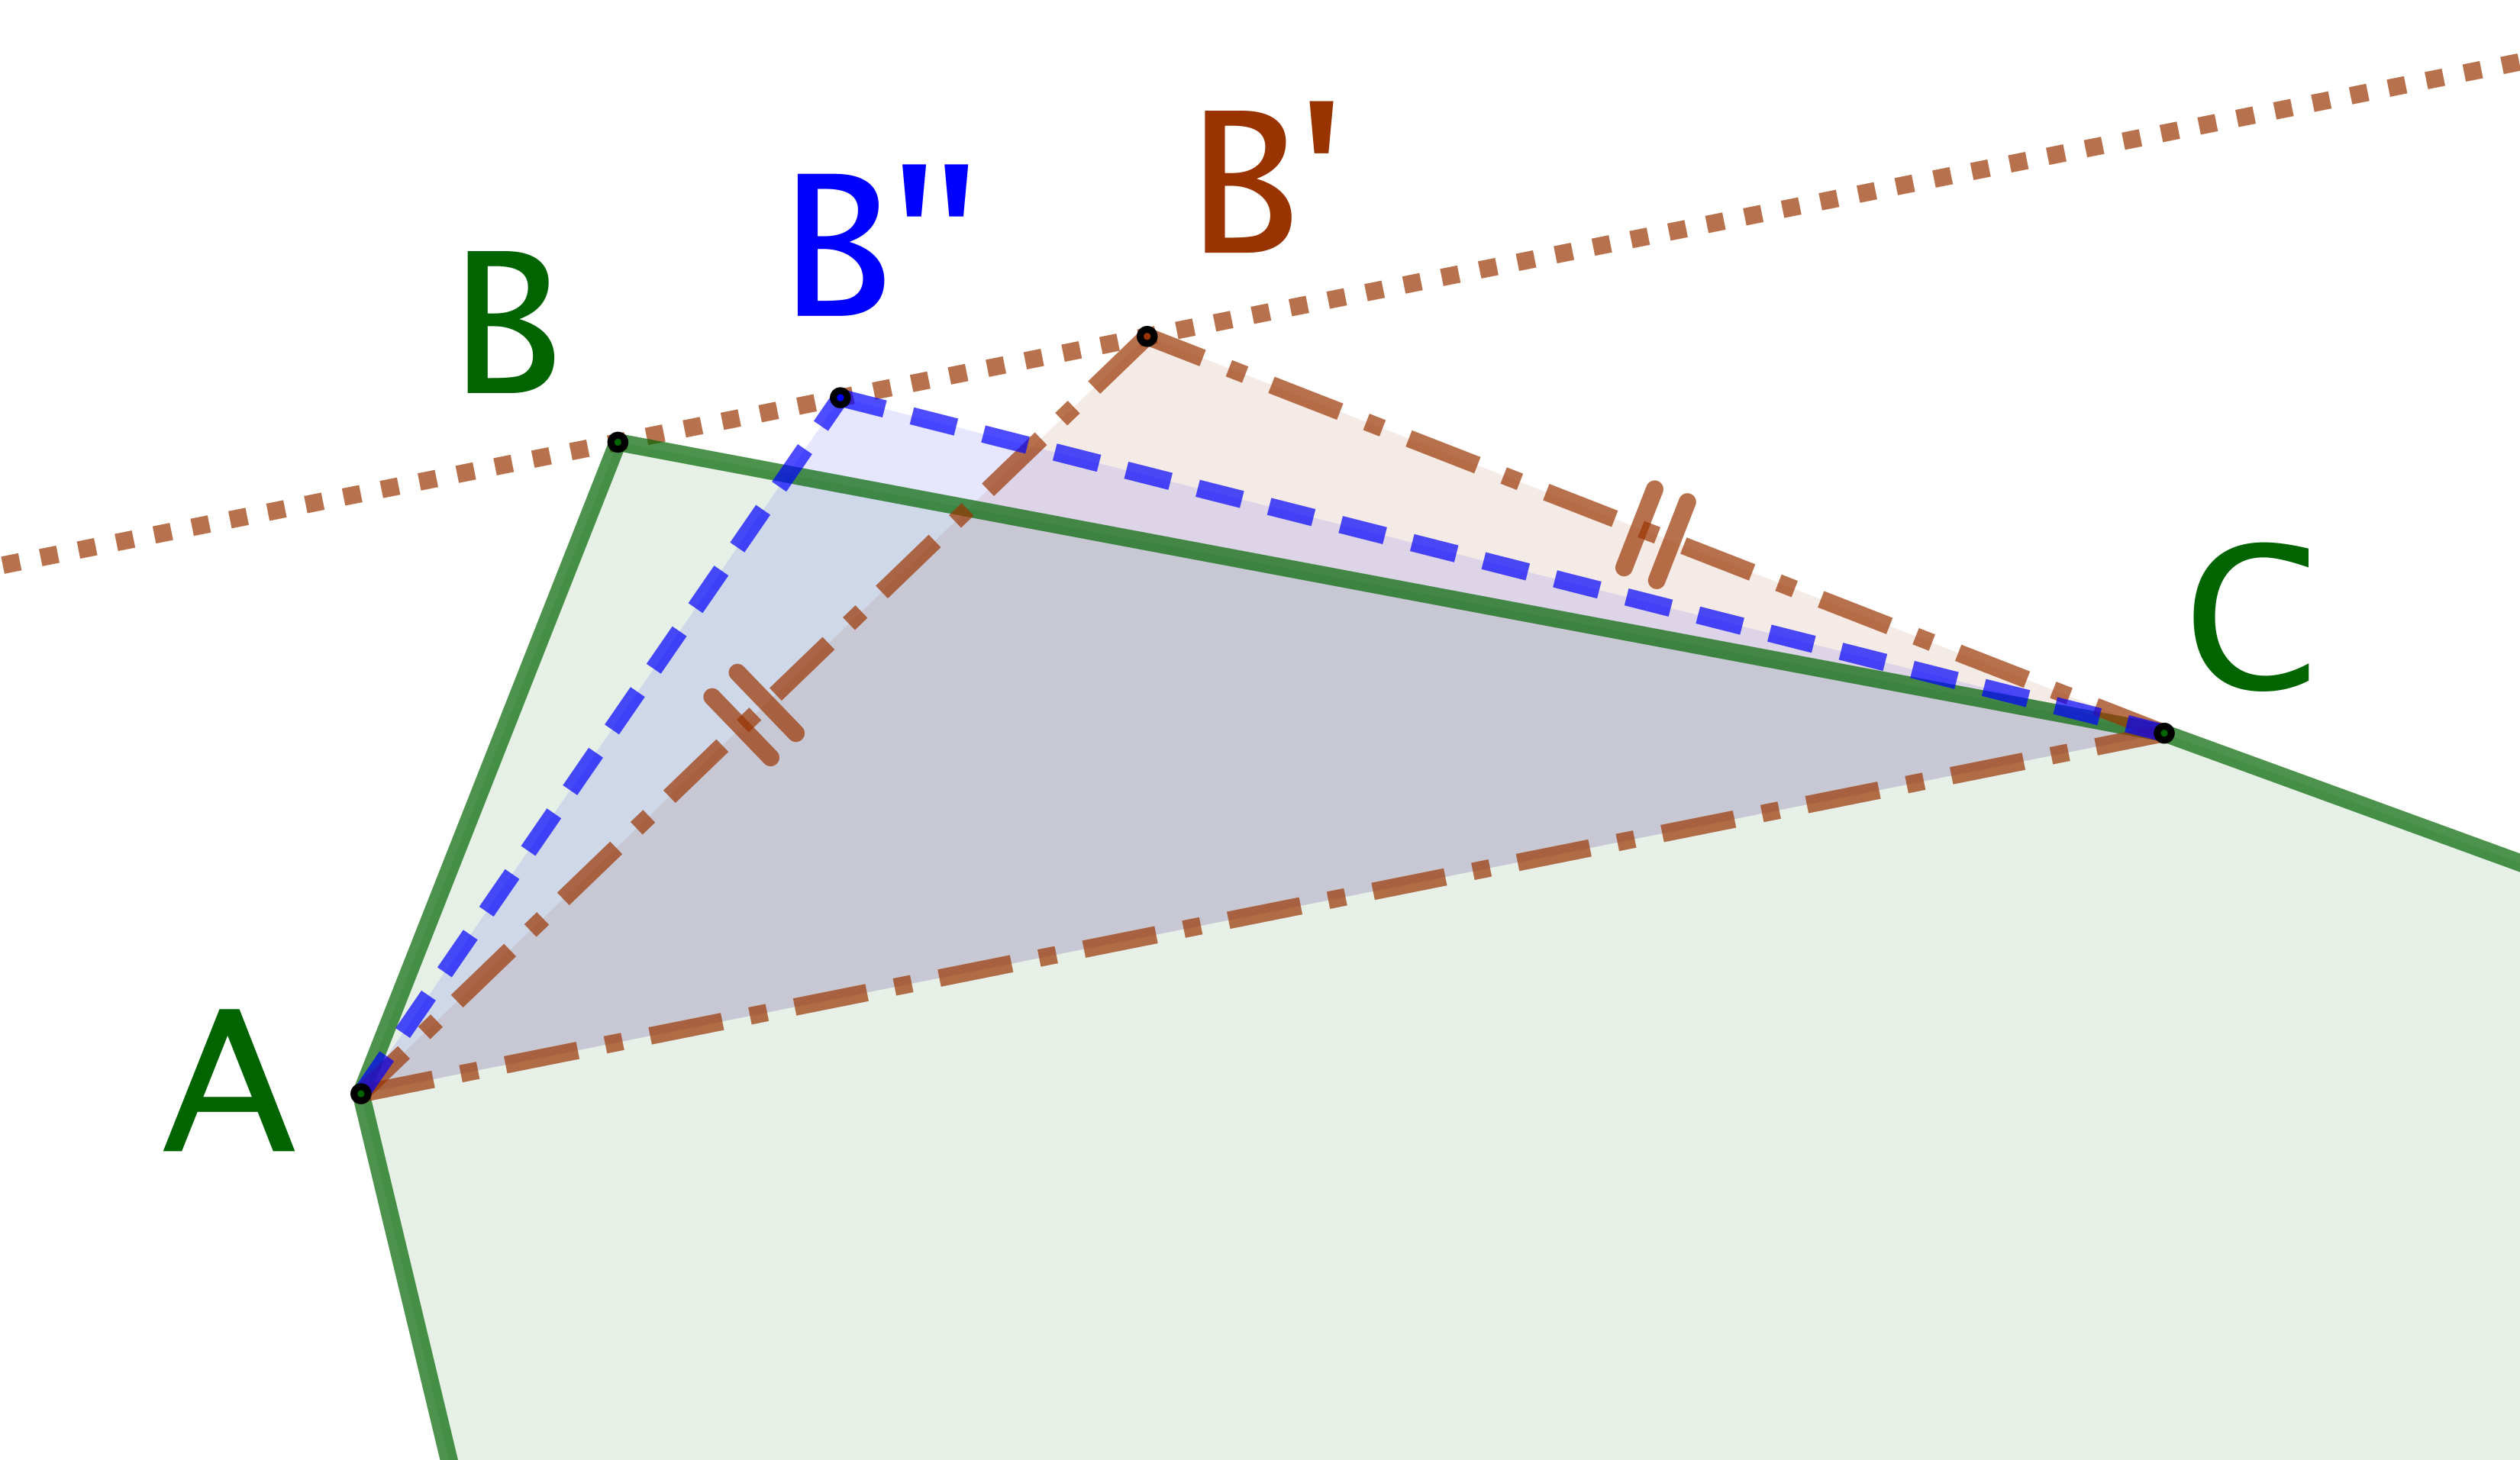
\includegraphics[scale=.4]{content/polygon/sol-is/not-iso-KO.png}
%	\end{multicols}
%
%	Dans chaque cas, nous avons construit un \ngone\ convexe $\setproba{P}^{\,\prime\prime}$ tel que
%	$\cyclelen{\setproba{P}^{\,\prime\prime}} < \cyclelen{\setproba{P}}$
%	et
%	$\area{\setproba{P}^{\,\prime\prime}} = \area{\setproba{P}}$.
%	Un simple agrandissement donne un \ngone\ convexe $\setproba{P}^{\,\prime}$ vérifiant
%	$\cyclelen{\setproba{P}^{\,\prime}} = \cyclelen{\setproba{P}}$
%	et
%	$\area{\setproba{P}^{\,\prime}} > \area{\setproba{P}}$.
%\end{proof}
%
%
%\begin{remark}
%	Le fait précédent ne permet pas de se ramener toujours au cas d'un \nequi\ convexe. Il nous dit juste que si un \ngone\ convexe maximise son aire à périmètre fixé, alors il devra être, a minima, un \nequi. La nuance est importante, et une similaire existe pour la conclusion du fait suivant.
%\end{remark}
%
%
%% ----------------------- %
%
%
%\begin{fact} \label{almost-reg-poly}
%	Si un \nequi\ convexe $\setproba{P}$ n'est pas un \niso,
%	alors il existe un \ngone\ convexe $\setproba{P}^{\,\prime}$ tel que
%	$\cyclelen{\setproba{P}^{\,\prime}} = \cyclelen{\setproba{P}}$
%	et
%	$\area{\setproba{P}^{\,\prime}} > \area{\setproba{P}}$.
%\end{fact}
%
%
%\begin{proof}
%	Par hypothèse, nous avons deux paires de côtés
%	$\big( [AB] , [BC] \big)$ et
%	$\big( [DE] , [EF] \big)$ telles que
%	$\anglein{BAC} > \anglein{DEF}$ comme ci-dessous, sans savoir si un côté lie les sommets $C$ et $D$, et de même pour $F$ et $A$.
%	Par contre, il est possible que $C$ et $D$ soient confondus.
%	%
%	\begin{multicols}{2}
%		\centering
%		
%		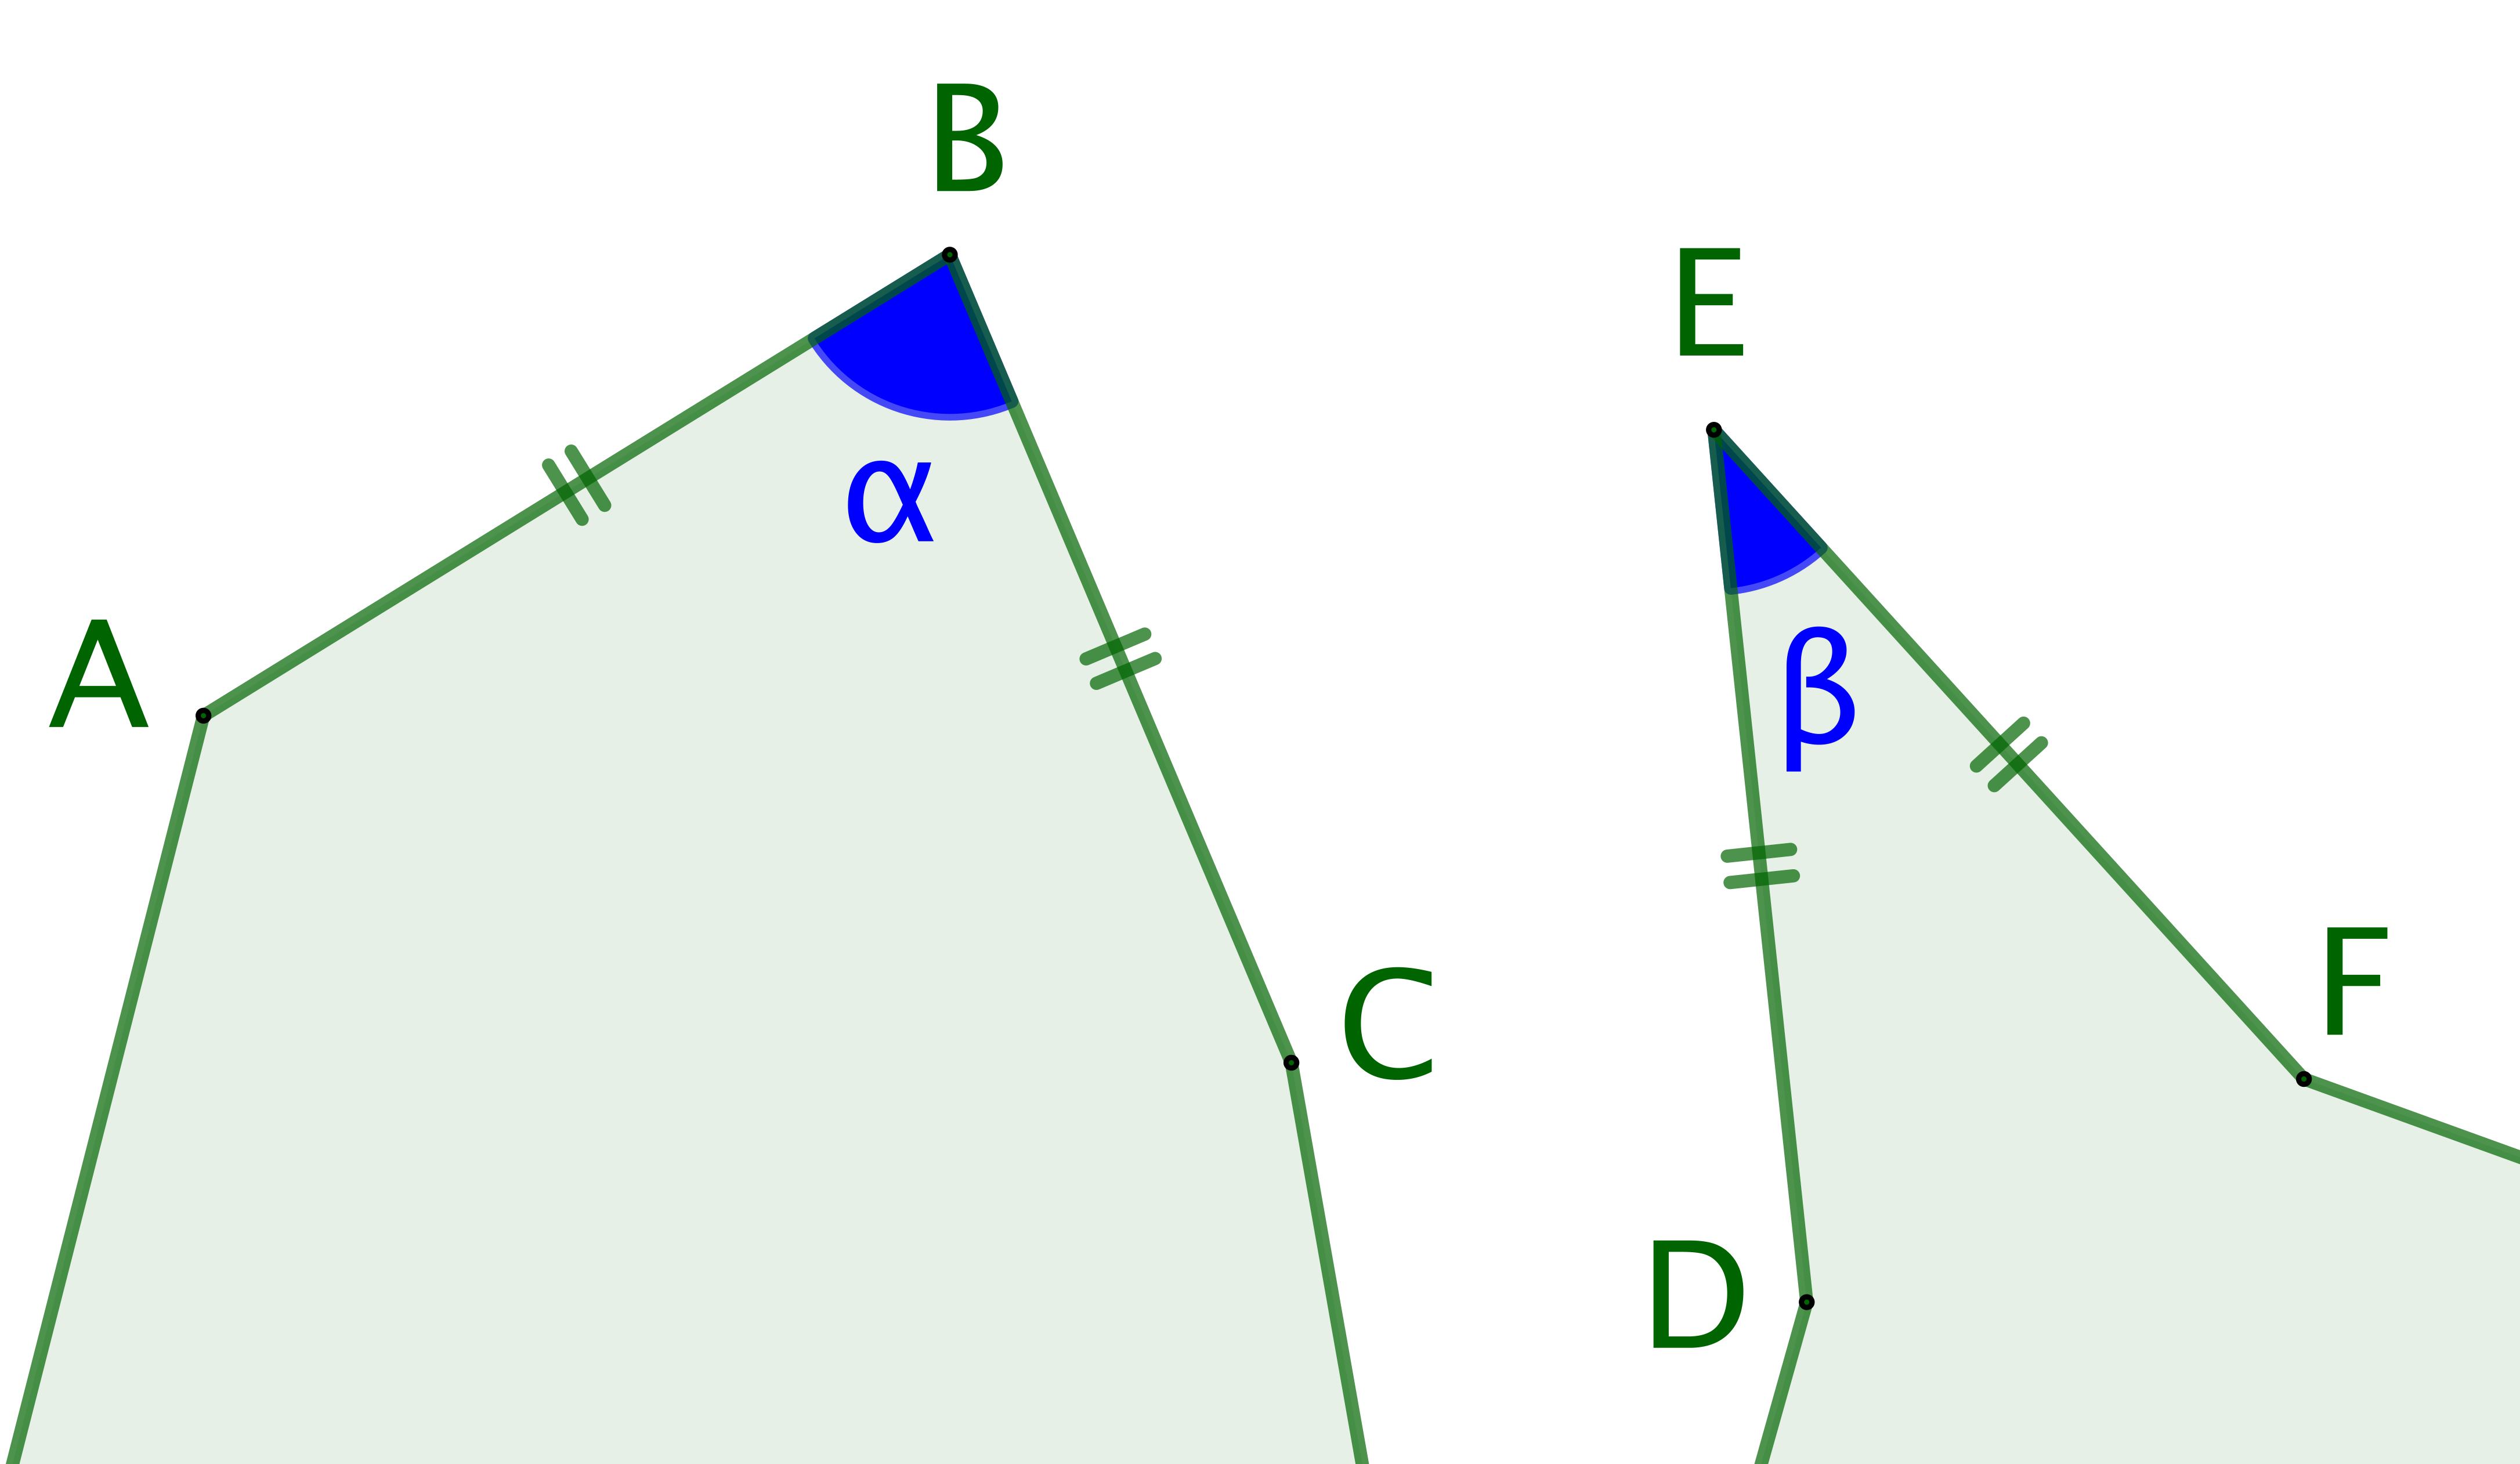
\includegraphics[scale=.4]{content/polygon/sol-is/2-eq-angles-start.png}
%		
%		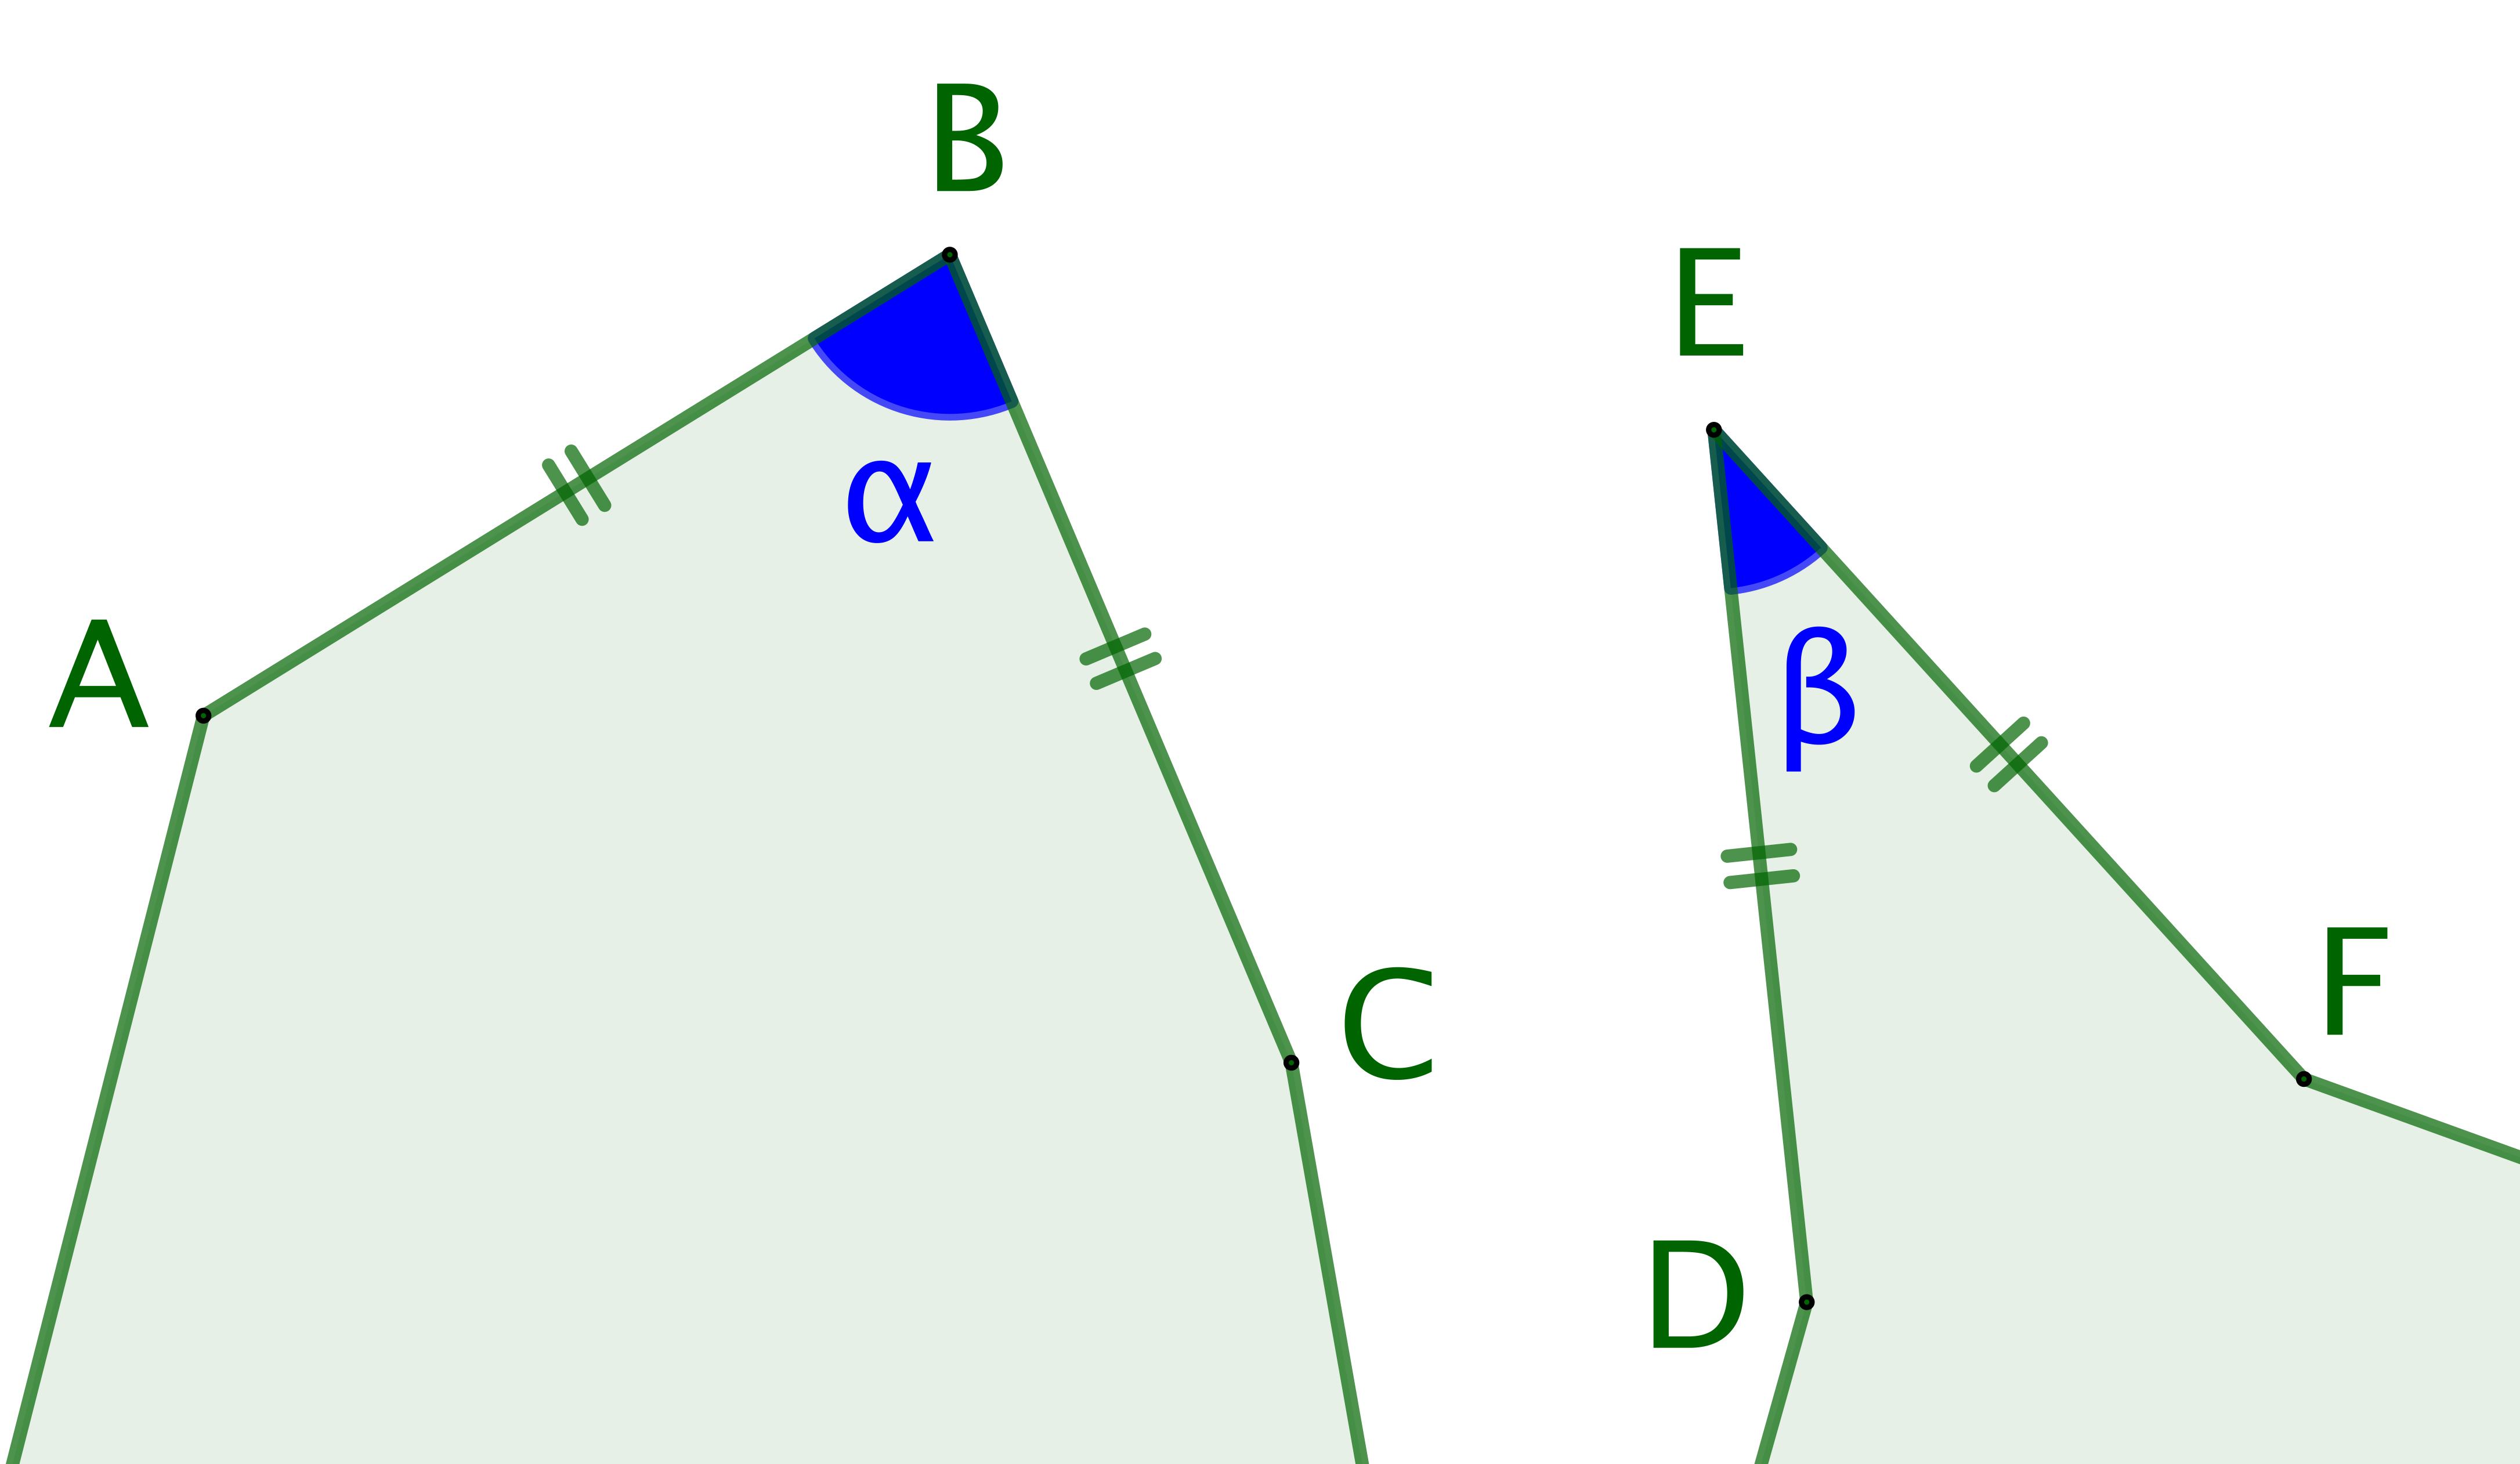
\includegraphics[scale=.4]{content/polygon/sol-is/2-eq-angles-start.png}
%	\end{multicols}
%	
%	
%	
%	\newpage
%	
%
%
%
%
%	
%	Dans nos manipulations à venir, nous fixons $A$, $C$, $E$ et $G$, tout en cherchant à bouger $B$ et $F$ de sorte à toujours avoir des triangles isocèles \og \emph{pointant} \fg\ vers l'extérieur du convexe $\setproba{P}$.
%	Posons $\ell = AB$, $d_1 = AC$ et $d_2 = EG$. Comme nous ne touchons pas aux points $A$, $C$, $E$ et $G$, les nombres $d_1$ et $d_2$ sont constants.
%	%
%	\begin{itemize}
%		\item ????
%
%		\item ????
%	\end{itemize}
%
%
%	FAUX 
%	Les deux exemples ci-dessus nous permettent de noter que si $\alpha = \anglein{ABC}$ diminue, et $\beta = \anglein{EFG}$ augmente, alors la somme des aires se rapprochent de $0$.
%	Par raison de symétrie, si on fixe $\anglein{ABC} + \anglein{EFG}$, on devine que la somme des aires est maximisée quand $\anglein{ABC} = \anglein{EFG}$.
%	Nous allons établir ceci de façon élémentaire en commençant par les calculs suivants où
%	$\ell = AB$,
%	$\mu = \frac{\alpha + \beta}{2}$ et
%	$\delta = \mu - \beta > 0$ (rappelons que nous avons supposé $\alpha > \beta$).
%
%	\medskip
%	\begin{stepcalc}[style=ar*]
%		\area{ABC} + \area{EFG}
%	\explnext*{Formule dite des sinus.}{}
%		\dfrac12 BA \cdot BC \cdot \sin \big( \anglein{ABC} \big)
%		+
%		\dfrac12 FE \cdot FG \cdot \sin \big( \anglein{EFG} \big)
%	\explnext{}
%		\dfrac12 \ell^2 ( \sin \alpha + \sin \beta )
%	\explnext*{Formules de Simpson.}{}
%		\dfrac12 \ell^2 \sin \big( \dfrac{\alpha + \beta}{2} \big) \cos \big( \dfrac{\alpha - \beta}{2} \big)
%	\explnext{}
%		\dfrac12 \ell^2 \sin \mu \cos \delta
%	\end{stepcalc}
%
%
%	\medskip
%
%	Comme $(\delta ; \mu) \in \intervalO{0}{\pi}^2$,
%	nous avons $\sin \mu \cos \delta > \sin \mu$.
%	Remplaçons alors $\alpha$ et $\beta$ respectivement par $\alpha^{\,\prime}$ et $\beta^{\,\prime}$ de telle sorte que $\alpha^{\,\prime} = \beta^{\,\prime} = \frac{\alpha + \beta}{2} = \mu$.
%	Notons que
%	$0 < \beta < \mu < \alpha < \pi$
%	(diminution de $\alpha$ et augmentation de $\beta$).
%	Deux situations se présentent à nous.
%	%
%	\begin{itemize}
%		\item Le \ngone\ obtenu ne perd aucun côté.
%		Comme la convexité est gardée, c'est gagné.
%
%		\item Le \ngone\ obtenu perd au moins un côté. La solution consiste à choisir
%		$\alpha^{\,\prime\prime} = \mu + \frac{\delta}{2}$ et $\beta^{\,\prime\prime} = \mu - \frac{\delta}{2}$
%		au lieu de
%		$\alpha^{\,\prime} = \beta^{\,\prime} = \mu$, puisque nous avons
%		$\cos \delta < \cos \big( \frac{\delta}{2} \big)$ et
%		$0 < \beta < \beta^{\,\prime\prime} < \mu < \alpha^{\,\prime\prime} < \alpha < \pi$.
%	\end{itemize}
%\end{proof}
%
%
%\begin{remark}
%	Une démonstration géométrique courante du fait précédent, que l'on retrouve souvent reproduite, s'appuie sur un résultat attribué à Zénodore sur la maximisation de l'aire totale de deux triangles isocèles de bases fixées, et de périmètre total constant:
%	ce résultat affirme que les deux triangles doivent avoir des angles en leur sommet principal de même mesure.
%	Malheureusement, cette preuve échoue lors de la disparition d'un sommet en choisissant les deux triangles isocèles optimaux pour construire un nouveau \ngone\ \og plus gros \fg\,, sauf à affiner la recherche comme dans notre approche analytique.
%	Indiquons, au passage, que la preuve du résultat de Zénodore est un peu fastidieuse, sans être ingrate.
%\end{remark}
%	
%
%% ----------------------- %
%
%
%%\begin{remark}
%%	La méthode des extrema liés, rappelée dans la remarque \ref{constrained-extrema}, donne une autre justification. Voici comment faire.
%%	%
%%	\begin{itemize}
%%		\item $\area{ABC} + \area{EFG} = \frac14 ( d_1^2 \tan \alpha + d_2^2 \tan \beta )$
%%
%%		\item
%%		\begin{stepcalc}[style=sar]
%%			4 \ell
%%		\explnext{}
%%			AB + BC + EF + FG
%%		\explnext{}
%%			2 ( AB + EF )
%%		\explnext{}
%%			\frac{d_1}{\cos \alpha} + \frac{d_2}{\cos \beta}
%%		\end{stepcalc}
%%
%%		\item Pour $(\alpha ; \beta) \in \intervalO{0}{\frac{\pi}{2}}^2$, on cherche donc à maximiser $f(\alpha ; \beta) =  d_1^2 \tan \alpha + d_2^2 \tan \beta$ sous la contrainte $g(\alpha ; \beta) = 0$ où $g(\alpha ; \beta) = 4 \ell - \frac{d_1}{\cos \alpha} - \frac{d_2}{\cos \beta}$.
%%
%%		\item On doit avoir $\lambda \in \RR$ tel que
%%    	$\pder[i]{f}{\alpha}{1} = \lambda \pder[i]{g}{\alpha}{1}$ et
%%    	$\pder[i]{f}{\beta}{1} = \lambda \pder[i]{g}{\beta}{1}$
%%		(méthode des extrema liés).
%%
%%		\item Donc
%%    	$\frac{d_1^2}{\cos^2 \alpha} = \lambda \frac{d_1 \sin \alpha}{\cos^2 \alpha}$,
%%		c'est-à-dire
%%		$\lambda \sin \alpha = d_1$.
%%		De même,
%%		$\lambda \sin \beta = d_2$.
%%	
%%		\item ????
%%	\end{itemize}
%%\end{remark}
%
%
%% ----------------------- %
%
%
%\begin{fact} \label{nece-cond}
%	Si un \ngone\ $\setproba{P}$ n'est pas régulier,
%	alors il existe un \ngone\ convexe $\setproba{P}^{\,\prime}$ tel que
%	$\cyclelen{\setproba{P}^{\,\prime}} = \cyclelen{\setproba{P}}$
%	et
%	$\area{\setproba{P}^{\,\prime}} > \area{\setproba{P}}$.
%\end{fact}
%
%
%\begin{proof}
%	Le fait \ref{max-is-conv} permet de considérer le problème de maximisation d'aire à longueur fixée juste pour des \ngones\ convexes.
%	Selon les faits \ref{iso-poly} et \ref{almost-reg-poly}, si, parmi les \ngones\ convexes de longueur fixée, il en existe un d'aire maximale, alors il devra être, a minima, régulier.
%\end{proof}
